% NB: use pdflatex to compile NOT pdftex.  Also make sure youngtab is
% there...

% converting eps graphics to pdf with ps2pdf generates way too much
% whitespace in the resulting pdf, so crop with pdfcrop
% cf. http://www.cora.nwra.com/~stockwel/rgspages/pdftips/pdftips.shtml

\documentclass[10pt,aspectratio=169,dvipsnames]{beamer}
\usetheme[color/block=transparent]{metropolis}

\usepackage[absolute,overlay]{textpos}
\usepackage{booktabs}
\usepackage[utf8]{inputenc}
\usepackage{tikz}
\usetikzlibrary{arrows.meta}

\usepackage[europeanresistors,americaninductors]{circuitikz}
\usepackage[scale=2]{ccicons}
\usepackage[official]{eurosym}

%use this to add space between rows
\newcommand{\ra}[1]{\renewcommand{\arraystretch}{#1}}
\newcommand{\hrefc}[2]{\href{#1}{\bf\color{blue}{\underline{#2}}}}
\newcommand{\urlc}[1]{\hrefc{#1}{#1}}

%doesn't work for reasons I don't understand
%\renewcommand{\href}[2]{\href{#1}{\bf\color{blue}{\underline{#2}}
%\renewcommand{\url}[1]{\href{#1}{#1}}

\xdefinecolor{TUred}{RGB}{197,14,31}

\setbeamerfont{alerted text}{series=\bfseries}
\setbeamercolor{alerted text}{fg=TUred}
\setbeamercolor{background canvas}{bg=white}
\setbeamercolor{frametitle}{bg=lightgray!40, fg=TUred}
\setbeamercolor{title}{fg=TUred}

\addtobeamertemplate{frametitle}{}{%
  \begin{textblock*}{100mm}(1.01\textwidth,2pt)
    
\includegraphics[width=1.5cm]{images/TUB.png}
    \end{textblock*}}

\newcommand{\R}{\mathbb{R}}

\def\l{\lambda}
\def\m{\mu}
\def\d{\partial}
\def\cL{\mathcal{L}}
\def\co2{CO${}_2$}

\def\el{${}_{el}$}
\def\th{${}_{th}$}
\def\gas{${}_{gas}$}

\newcommand{\ubar}[1]{\text{\b{$#1$}}}

% for sources http://tex.stackexchange.com/questions/48473/best-way-to-give-sources-of-images-used-in-a-beamer-presentation

\setbeamercolor{framesource}{fg=gray}
\setbeamerfont{framesource}{size=\tiny}

\newcommand{\source}[1]{\begin{textblock*}{5cm}(10.5cm,8.35cm)
    \begin{beamercolorbox}[ht=0.5cm,right]{framesource}
        \usebeamerfont{framesource}\usebeamercolor[fg]{framesource} {#1}
    \end{beamercolorbox}
\end{textblock*}}

\usepackage{hyperref}

%\usepackage[pdftex]{graphicx}

\graphicspath{{../graphics/}}

\DeclareGraphicsExtensions{.pdf,.jpeg,.png,.jpg}


\def\goat#1{{\scriptsize\color{green}{[#1]}}}
\let\olditem\item
\renewcommand{\item}{%
\olditem\vspace{5pt}}


\title{System-level impacts of 24/7 carbon-free electricity procurement in Europe}

%\subtitle{---}
\author{
  Iegor Riepin, Tom Brown\\
  \hrefc{https://tub-ensys.github.io/}{Department of Digital Transformation in Energy Systems}, TU Berlin
}

\date{11 October 2022}

\titlegraphic{%
  \vspace{0cm}
  \hspace{10.7cm}
    
\includegraphics[trim=0 0cm 0 0cm,height=1.2cm,clip=true]{images/TUB.png}

\vspace{5.1cm}
   
}

\begin{document}

\maketitle


\begin{frame}
  \frametitle{Acknowledgements}

  \begin{itemize}
    \item {\bf Funding:} This study was supported by a grant from Google, Inc. 
    \item {\bf Acknowledgements:} The authors thank members of the Google energy markets and policy team 
    for their feedback and inputs on earlier drafts of this report. 
    We also thank the \hrefc{https://pypsa.org/}{PyPSA team} and many contributors to the open-source 
    PyPSA energy system modelling tool used in this study (see: \hrefc{https://github.com/PyPSA/PyPSA}{github.com/PyPSA})
    \item 
    {\bf Copyright} Unless otherwise stated, graphics and text are Copyright \copyright Tom Brown and Iegor Riepin, 2022.
    Graphics and text for which no other attribution are given are licensed under a 
    \href{https://creativecommons.org/licenses/by/4.0/}{CC BY 4.0}.  {\footnotesize \ccby} 
    \item The content of this study, including any errors or omissions, are the responsibility
    of the authors alone.
  \end{itemize}

\end{frame}


\begin{frame}

  \frametitle{Table of Contents}
  \setbeamertemplate{section in toc}[sections numbered]
  \tableofcontents[hideallsubsections]
\end{frame}


%----------------------------------------
%----------------------------------------

\section{Introduction}


\begin{frame}{Introduction}

  \centering
    \begin{itemize}
    \item Climate change is driving a global effort to rapidly decarbonise 
    electricity systems across the globe. 
    Many public and private energy buyers have joined this effort 
    by purchasing certificates for renewable energy or
    by procuring renewable energy directly with Power Purchase Agreements (PPAs).
    \item Such \alert{voluntary commitments accelerate the deployment of renewable 
    capacity} above the policy requirements in the countries and jurisdictions
    where these companies operate, facilitating faster
    transformation of electricity markets.
    \item Additionally, many early actors in the field have paved the way for others to follow 
    \hrefc{https://www.gstatic.com/gumdrop/sustainability/247-carbon-free-energy.pdf}{by 
    developing methods and establishing standard contracts} for clean energy procurement.
    \end{itemize}
  
\end{frame}



\begin{frame}{Introduction}

  \begin{columns}[T]
    \begin{column}{6cm}
      \begin{itemize}
        \item   PPAs typically are typically used for renewable energy to match generation 
        and consumption on average over a year.
        \item For example, more than 370 members of the \href{https://www.there100.org/}{RE100} group have committed to purchasing enough renewable energy to match
        \alert{100\% of their electricity consumption on an annual basis}.
      \end{itemize}
    \end{column}

  \begin{column}{10cm}
      \centering
      
      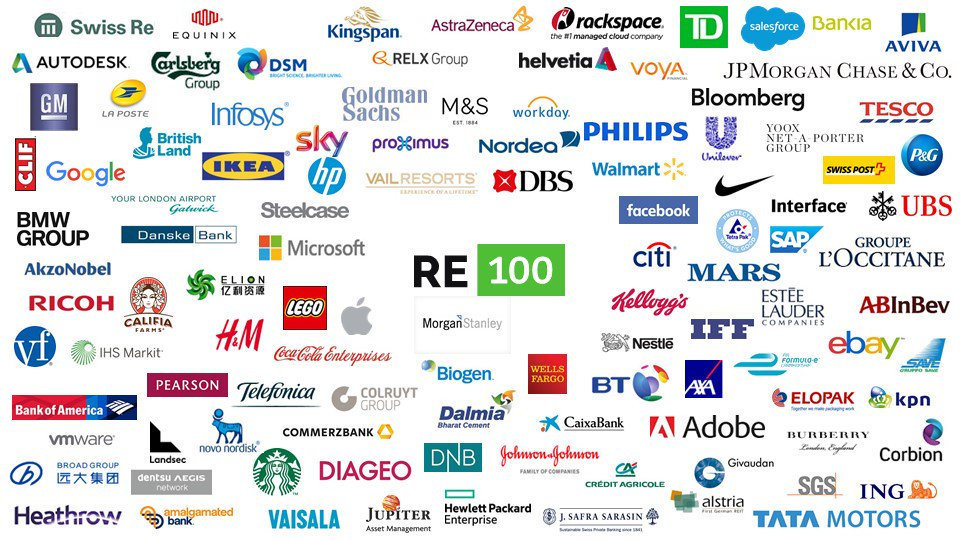
\includegraphics[width=10cm]{images/100re-companies.jpg}
      \vspace{.1cm}
      {\footnotesize
      More than 370 companies have joined \hrefc{https://www.there100.org/}{RE100}
      }
    \end{column}
    \end{columns}

    \source{source: \href{https://www.there100.org/}{RE100}}
\end{frame}
  


\begin{frame}{Introduction}
  
    \begin{itemize}
    \item However, electricity buyers that commit to 100\% annual matching 
    from renewable energy sources still face times when generation 
    from wind and solar generators is not sufficient to match 
    the companies’ electricity demand. 
    \item Thus, although buyers match their demand on a \alert{yearly} basis with 
    renewable energy, on an \alert{hourly} basis they still have hours 
    when they have to rely on carbon-emitting technologies available 
    on the local market, such as coal and gas-fired power plants.
    \end{itemize}

  \centering
  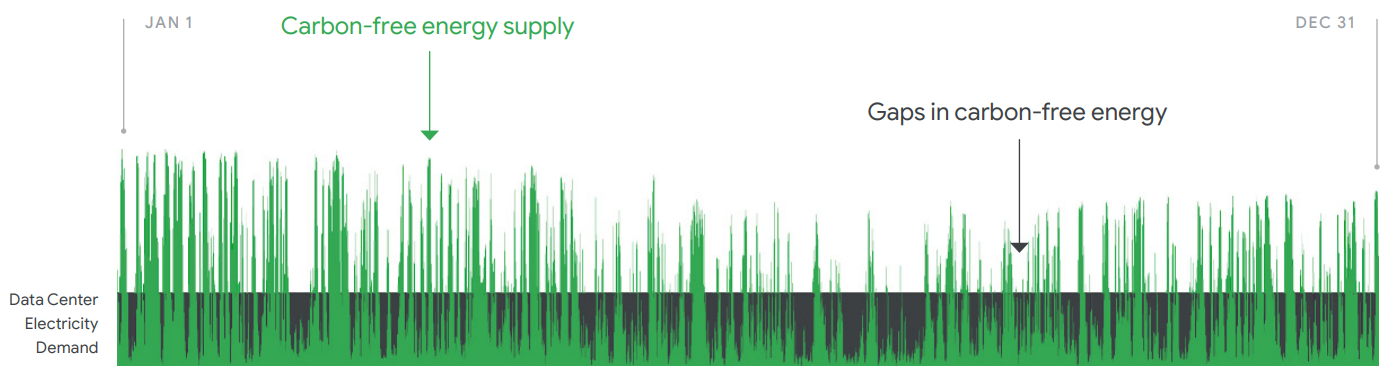
\includegraphics[width=14cm]{images/google-year.png}
  \source{\href{https://www.gstatic.com/gumdrop/sustainability/247-carbon-free-energy.pdf}{source: Google 2021, 24/7 CFE: Methodologies and Metrics}}
           
\end{frame}



\begin{frame}{Introduction}
  
  More generally, 100\% annual matching leads to many challenges 
  from the electricity buyers' and system perspectives: 
  \begin{itemize}
  \item No \alert{simultaneity} - variable generation of wind and solar power is not aligned with the 
  buyers' electricity consumption profile.
  \item Lack of \alert{additionality} - some buyers procure unbundled guarantees of origin from existing 
  facilities, which does not lead to additional renewable generation.
  \item Displaced \alert{location} - some buyers procure PPAs from locations far away 
  from their consumption, where there is no way to transmit the electricity to the demand.
  \item Exposure to \alert{risk} - electricity buyers are exposed to price volatility 
  in local electricity markets, since they still have to procure electricity to cover
  the difference between demand and supply.
  \item Need for \alert{backup} - the rest of the electricity system still has to 
  maintain backup and flexibility options for hours with low renewable generation.
  \end{itemize}
  
\end{frame}



\begin{frame}{24/7 carbon-free energy}

  \centering

  There is growing interest from leaders in voluntary clean
  electricity procurement to cover their consumption 
  with clean energy supply on a \alert{truly 24/7 basis}. \\
  \vspace{0.3cm}
  Achieving 24/7 Carbon-Free Energy (CFE) means that every kilowatt-hour of electricity consumption is met
  with carbon-free electricity sources, \alert{every hour of every day}.
  
\end{frame}



\begin{frame}{Yearly versus hourly matching}
  
  24/7 CFE procurement has potential benefits over the 100\% renewable matching:
  
  \begin{itemize}
  \item Ensure match of electricity consumption with carbon-free resources 
        on an \alert{hourly basis}.
  \item Enable much \alert{deeper reductions in CO$_2$ emissions} associated 
        to buyer's electricity consumption.
  \item Ensure that contracted power is \alert{additional} (i.e. leads to new capacity).
  \item Ensure that power comes from the \alert{same bidding zone}.
  \item Enable technology-neutral procurement of \alert{carbon-free} rather than renewable technologies 
        (such as advanced clean dispatchable power generation and long-duration energy storage).
  \end{itemize}
  
\end{frame}



\begin{frame}{24/7 carbon-free energy}
  
  \begin{columns}[T]
  \begin{column}{8cm}

    \begin{itemize}
    \item The \hrefc{https://www.un.org/en/energy-compacts/page/compact-247-carbon-free-energy}{24/7 Carbon-free Energy Compact} 
    initiative was launched in 2021 by Sustainable Energy for All and the United Nations. 
    It now includes more than 80 companies, policymakers, investors, and organizations 
    on a mission to realize a 24/7 Carbon-Free Energy future. 

    \item One of the front runners in the 24/7 initiative is Google Inc. In 2020 the company committed 
    \hrefc{https://www.gstatic.com/gumdrop/sustainability/247-carbon-free-energy.pdf}{to the goal} 
    of operating entirely on a 24/7-CFE approach at all its data centres and campuses worldwide by 2030. 
    Shortly after, Google published 
    \hrefc{https://www.gstatic.com/gumdrop/sustainability/policy-roadmap-carbon-free-energy.pdf}{a policy roadmap} 
    on achieving the 24/7-CFE goal.

    \end{itemize}
  \end{column}

  \begin{column}{8cm}
    \centering
    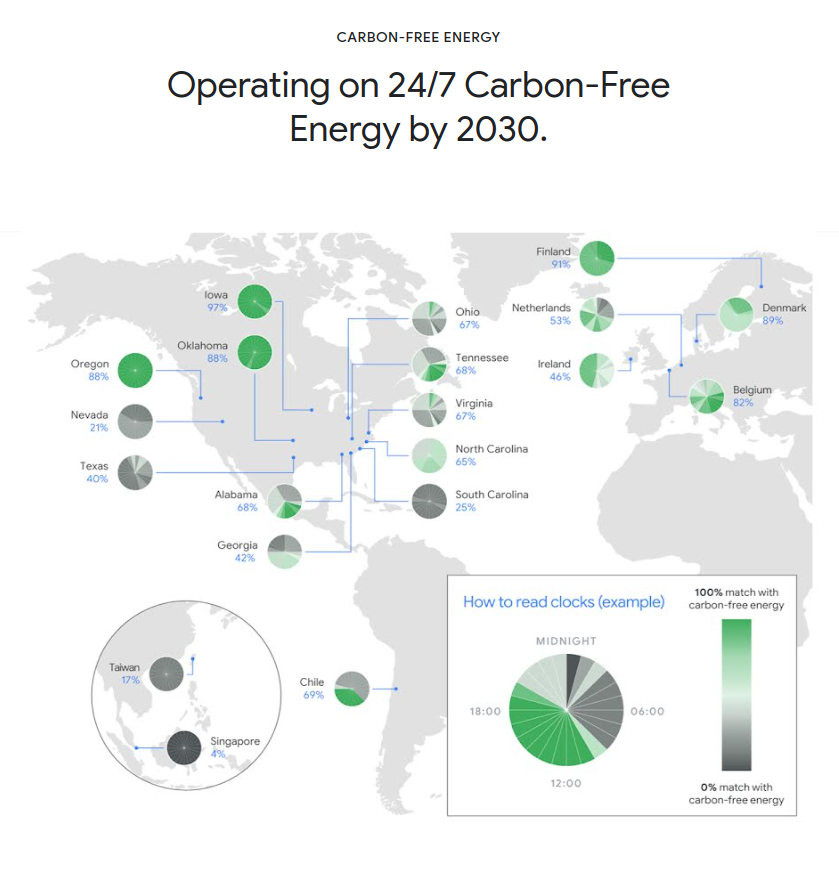
\includegraphics[width=7.5cm]{images/247-google-web.png}
    \vspace{.1cm}
  \end{column}

  \source{\href{https://sustainability.google/progress/energy/}{Google Inc.}}
  \end{columns}
  
\end{frame}



\begin{frame}{Focus of the study}

  In this study, we investigate both the \alert{means and costs of 24/7 procurement} 
  for companies in a selection of European countries 
  and the \alert{system impacts} for the rest of the European electricity system. 
  
  \vspace{0.3cm}
  In particular, we focus our analysis on the following quesitons:
    \begin{itemize}
    \item How can companies following 24/7~CFE procurement achieve hourly matching?
    \item What is the cost premium of 24/7~CFE versus 100\% annual matching?
    \item To what extent can technologies, such as long-duration storage or advanced dispatchable
          clean generators, help to achieve the 24/7~CFE goal?
    \item To which extent can 24/7~CFE contribute to reductions in CO$_2$
          emissions intensity of buyers' consumption? 
    \item If many companies follow the 24/7~CFE approach, how does this affect 
    emissions and flexibility needs in the rest of the electricity system?
    \end{itemize}

\end{frame}



\begin{frame}{Summary of key findings}

  \centering
  {\small

  \noindent\fbox{%
  \parbox{\textwidth}{%
    \begin{enumerate}

    \item 24/7~carbon-free energy (CFE) procurement leads to lower emissions for both the buyer and the system,
      as well as reducing the needs for flexibility in the rest of the system.  

    \item Reaching CFE for 90-95\% of the time can be done with only a small cost premium compared to annually matching 
    100\% renewable energy. 90-95\% CFE can be met by supplementing wind and solar with battery storage.

    \item Reaching 100\% CFE target is possible but costly with existing renewable 
    and storage technologies, with costs increasing rapidly above 95\%.
    
    \item 100\% CFE target could have a much smaller cost premium if long duration storage or 
    clean dispatchable technologies like advanced geothermal are available.
    
    \item 24/7~CFE procurement would create an early market for the advanced technologies,
    stimulating innovation and learning from which the whole electricity system would benefit.
    
  \end{enumerate}
  }}
  
  These European study results align with \hrefc{https://acee.princeton.edu/24-7/}{a similar study} 
  done by Princeton University in 2021 \\ for regions in the United States.
  }
  
\end{frame}


%----------------------------------------
%----------------------------------------

\section{Methodology and study design}



\begin{frame}
  \frametitle{A quick overview}


{\small
  \begin{itemize}
    
    \item The mathematical model for this study is build upon 
    \hrefc{https://github.com/PyPSA/pypsa-eur}{PyPSA-Eur(-Sec)} --
    a widely-used open-source optimization model for the European energy system.

    \item We encode a set of new equations and routines into the PyPSA-Eur(-Sec),
    which allow for modelling a situation when some corporate \& industrial (C\&I) electricity consumers 
    commit to a voluntary clean energy procurement.

    \item We compare 100\% annual matching with renewable energy versus 
    different targets for hourly CFE matching.

    \item We place C\&I consumers committed to a clean energy procurement in a 
    selection of European countries: Germany, Denmark, Ireland and the Netherlands.
    These countries differ in patterns of electricity demand, renewable potentials,
    national energy and climate policies, legacy fleets of generation capacities, degree 
    of interconnectons, etc. Apart form that, we consider different C\&I participation rates, a wide palette 
    of CFE generation technologies available for 24/7 consumers, 
    and two years (2025 and 2030). These differences help to understand and generalize 
    the impacts of 24/7 CFE procurement.
    
  \end{itemize}
}

\end{frame}


\begin{frame}
  \frametitle{PyPSA: an energy systems modelling toolbox}

\begin{columns}[T]
\begin{column}{7cm}

{\small
  \begin{itemize}
  \item PyPSA (Python for Power System Analysis) is an open source toolbox 
  for for state-of-the-art energy system modelling.
  \item Fills gap between power flow software (e.g. PowerFactory,
  MATPOWER) and energy system planning software (e.g. TIMES, OSeMOSYS).
  \item PyPSA development and maintenance is coordinated by the TU Berlin,
  \hrefc{https://www.ensys.tu-berlin.de/}{Department of Energy Systems}.  
  \item PyPSA is used worldwide by dozens of research institutes and companies.\\
  See \hrefc{https://pypsa.readthedocs.io/en/latest/users.html}{list of users}.
  \end{itemize}
}

\end{column}

\begin{column}{9cm}

\centering
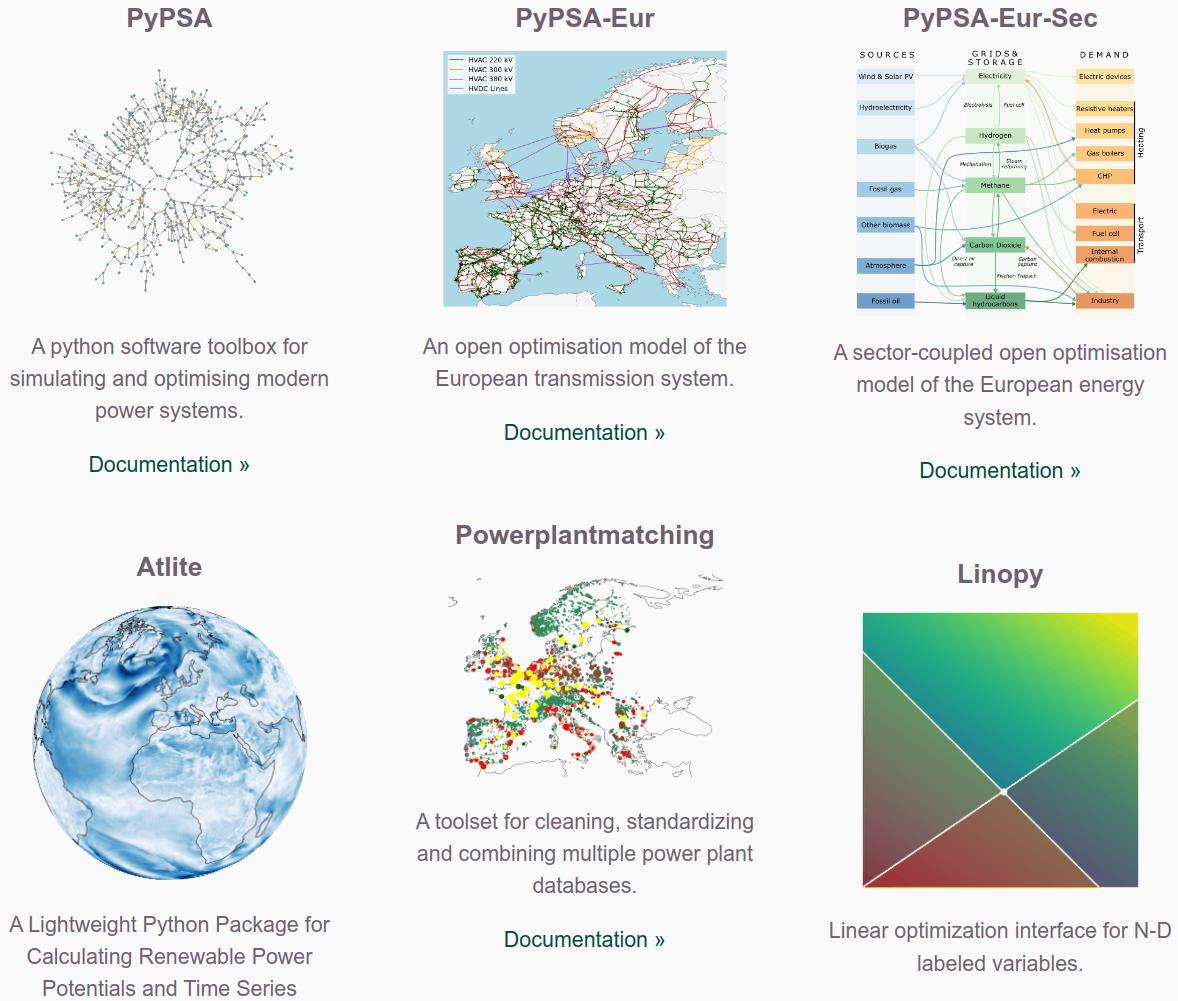
\includegraphics[width=8.5cm]{images/pypsa-web.png}
\source{\href{https://pypsa.org/}{PyPSA}}

\end{column}
\end{columns}

\end{frame}



\begin{frame}
  \frametitle{PyPSA-Eur(-Sec): open models of the European energy system}

  \begin{columns}[T]
  \begin{column}{7cm}
  {\small
  \begin{itemize}
  \item PyPSA-Eur is an open model of the European power system at the transmission network 
  level that covers the full ENTSO-E area.
  \item Only freely available and open data.
  \item Automated and configurable software pipeline from raw data to optimised electricity system.
  \item Adjustable temporal and spatial resolution.
  \item See \hrefc{https://pypsa-eur.readthedocs.io/en/latest/}{documentation}
  and \hrefc{https://docs.google.com/presentation/d/1mzj4X9uuO58gUvkhVMRCFWOJUWbs6NR9SNZe-RIkkNo/edit?usp=sharing}{feature summary} 
  for more details.
  \item PyPSA-Eur{\bf-Sec} version of the model adds building heating, transport and industry sectors, as well as gas networks.
  \end{itemize}
  }
  \end{column}

  \begin{column}{9cm}
    \centering
  {\footnotesize
    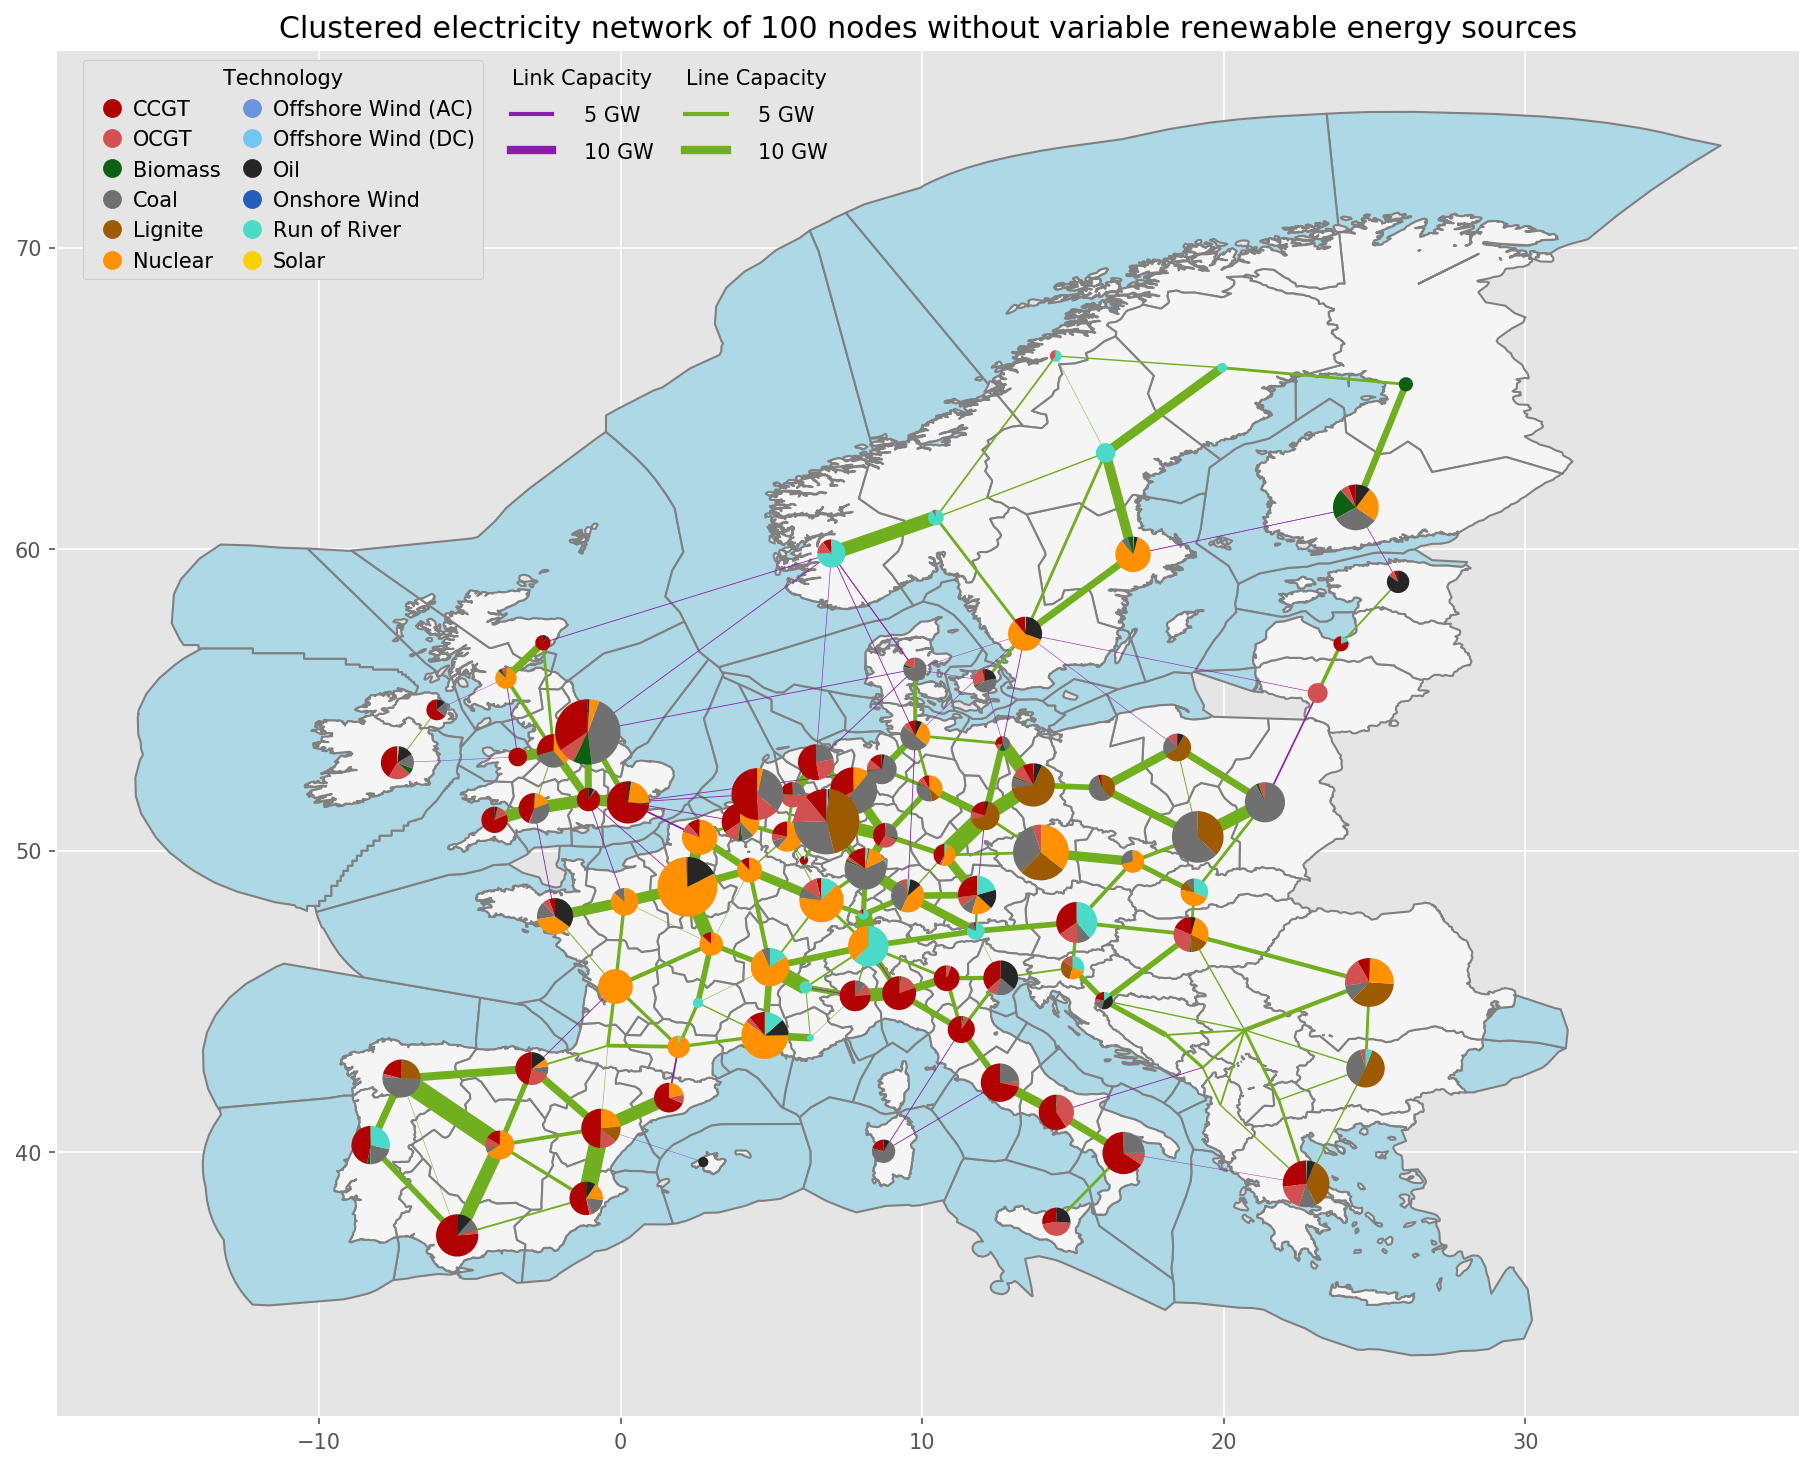
\includegraphics[width=8cm]{images/elec_s_100.png}
  
   \vspace{0.1cm}
   PyPSA-Eur(-Sec) suite of models are available on \hrefc{https://github.com/PyPSA}{GitHub}
  }
  \end{column}
  
  \end{columns}

\end{frame}



\begin{frame}{Modeling 24/7 CFE procurement}
  \begin{columns}[T]
  \begin{column}{7cm}
  {\small

  \begin{itemize}
  \item We implement a set of additional constraints to the PyPSA-Eur 
  to model a situation when a fraction of corporate and industry (C\&I) demand 
  commits to the 24/7~CFE procurement.
  \item The model optimises investment and operational decisions to meet projected
  electricity demand for the 24/7~CFE consumers, as well as
  the demand of other consumers in the European electricity system, while meeting all
  relevant engineering, reliability, and policy constraints.
  \end{itemize}
  }
  \end{column}

  \begin{column}{9cm}
  \centering
  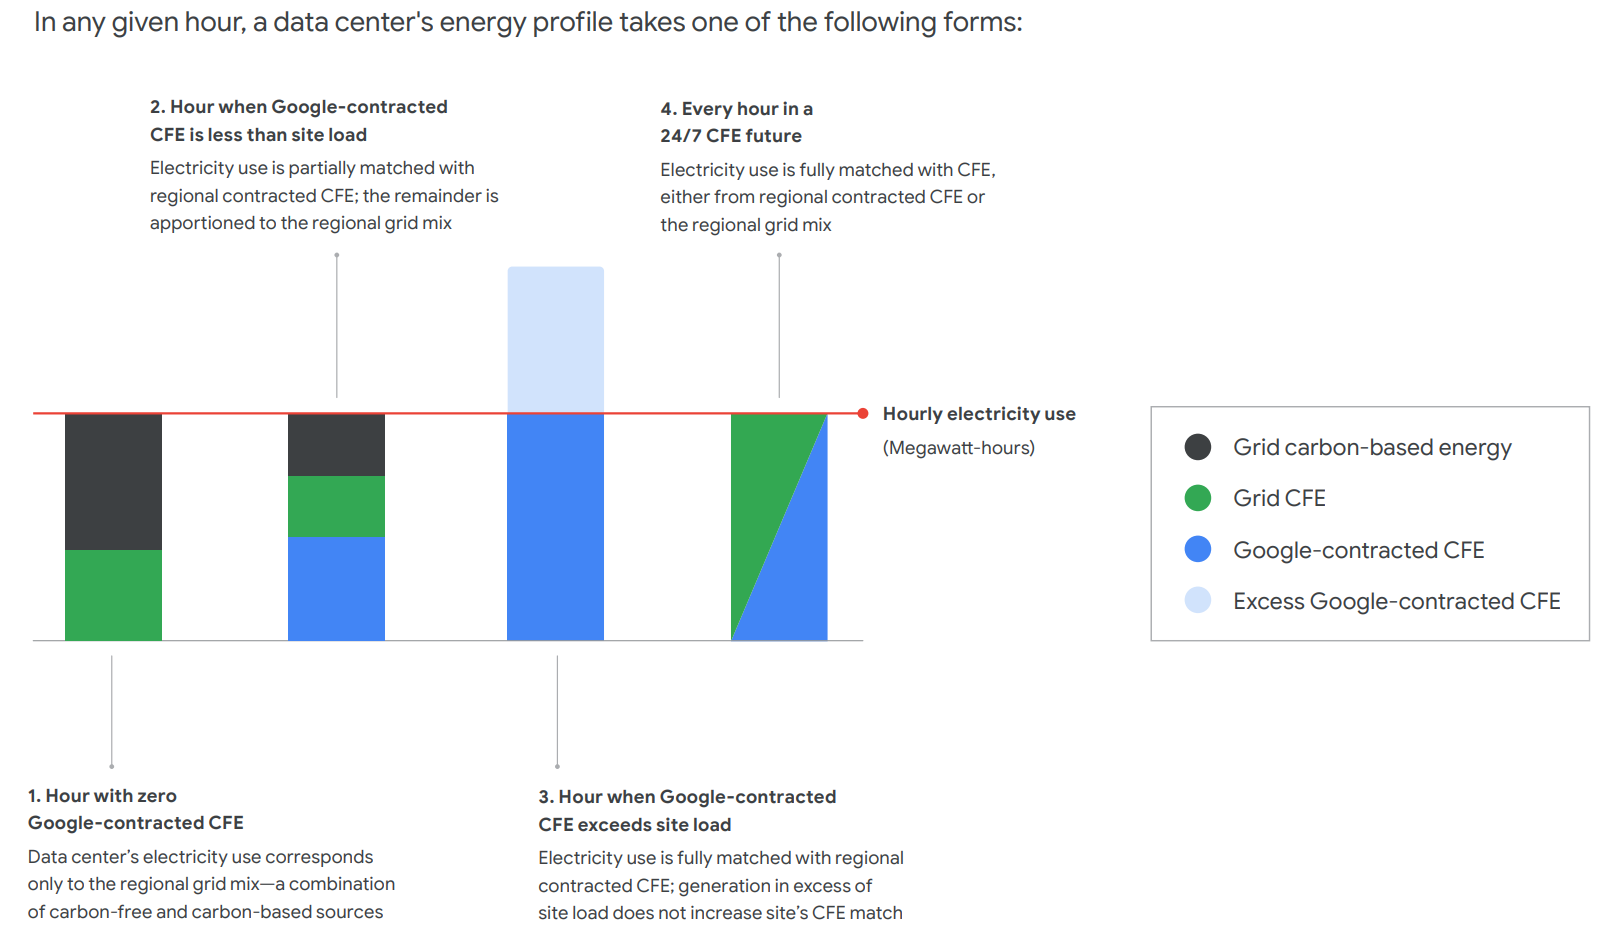
\includegraphics[width=8.5cm]{images/247-concept.png}
  {\footnotesize
  The methods are based on the Google's CFE procurement framework, presented in paper
  \hrefc{https://www.gstatic.com/gumdrop/sustainability/24x7-carbon-free-energy-methodologies-metrics.pdf}{"24/7 Carbon-Free Energy: Methodologies and Metrics"}
  }
  \source{\href{https://www.gstatic.com/gumdrop/sustainability/24x7-carbon-free-energy-methodologies-metrics.pdf}{source: Google 2021, 24/7 CFE: Methodologies and Metrics}}
  \end{column}

  \end{columns}

\end{frame}



\begin{frame}{Implementation of C\&I demand and supply}

  {\small

  The model optimizes a portfolio of carbon-free generation and storage technologies 
  procured by the participating C\&I consumers. The portfolio assets have to be located 
  in the same market zone.

  The hourly demand of C\&I consumers $d_t$ for hour $t$ can be met 
  by a combination of the following: \\
    \begin{itemize}
      \item dispatch $g_{r,t}$ of procured CFE generators $r\in CFE$ 
      \item dispatch $\bar{g}_{s,t}$ of procured storage technologies $s\in STO$
            (requires charge $\ubar{g}_{s,t}$)
      \item imports from the grid $im_t$.
    \end{itemize}
    }

\begin{columns}

  \begin{column}{7cm}
  \begin{equation*}
  \sum_{r\in CFE} g_{r,t} + \sum_{s\in STO} \left(\bar{g}_{s,t} - \ubar{g}_{s,t}\right) - ex_t + im_t  =  d_t \hspace{.7cm} \forall t
  \end{equation*}

  \vspace{0.3cm}
  {\small NB: the excess from the local supply $ex_t$ can either be sold to the grid 
  at market prices or curtailed.}
  \end{column}

\begin{column}{5cm}
\centering
\begin{circuitikz}
  \draw (0,13.5) to [short,i^=$im_t$]  (1.5,13.5) to (1.5,13);
  \draw [ultra thick] (0,13) node[anchor=south]{} -- (4,13);
  \draw(2.5,13) |- +(0,0.5) to [short,i^=$ex_t$] +(1.5,0.5);
  \draw (0.5,13) -- +(0,-0.5) node[sground]{};
  \draw (2,12) node[vsourcesinshape, rotate=270](V2){}
  (V2.left) -- +(0,0.6);
  \draw (3.5,13) -- (3.5,12.4);
  \draw (3.5,12.4) to [esource] (3.5,11.7);
  \draw (0.5,11) node{$d_t$};
  \draw (2,11) node{$g_{CFE,t}$};
  \draw (3.5,11) node{$g_{STO,t}$};
\end{circuitikz}
\end{column}

\end{columns}

\end{frame}



\begin{frame}{Implementation of 100\% annual matching}

  {\small
  
The \alert{100\% annual matching} is modelled with a constraint (\ref{eqn:RES100}), which requires C\&I consumers 
to purchase enough renewable electricity from the local bidding zone to match all of their electricity consumption
on an annual basis.

\vspace{0.3cm}
More formally, the sum of all dispatch $g_{r,t}$ for RES generators $r\in RES$ over the year $t\in T$ 
is equal to the annual demand $d_t$ of C\&I consumers:
  \begin{equation}
    \sum_{r\in RES, t\in T} g_{r,t} = \sum_{t\in T} d_t
  \label{eqn:RES100}
  \end{equation}
  }
\end{frame}


\begin{frame}{Implementation of 24/7 CFE matching}

  {\small

  The \alert{24/7 CFE matching} is modelled with a constraint (\ref{eqn:CFE}), 
  which matches demand of C\&I consumers with carbon-free resources on an hourly basis. 

  More formally, the constraint states that sum over generators from procured CFE resources $r\in CFE$,
  discharge and charge from storage technologies $s\in STO$,
  as well as import from the grid $im_t$ multiplied by the grid's CFE factor $CFE_t$
  must be higher or equal than a certain CFE target $x$ multiplied with the total load:
  \vspace{0.1cm}
  \begin{equation}
  \sum_{r\in CFE, t\in T} g_{r,t} + \sum_{s\in STO, t\in T} \left(\bar{g}_{s,t} - \ubar{g}_{s,t}\right) - \sum_{t\in T} ex_t + \sum_{t\in T} CFE_t \cdot im_t \geq x \cdot \sum_{t\in T} d_t
  \label{eqn:CFE}
  \end{equation}
  \vspace{0.1cm}
  \noindent\fbox{%
    \parbox{\textwidth}{%
  The \alert{CFE Score} $x$~[\%] measures the degree to which hourly electricity consumption 
  is matched with carbon-free electricity generation within the regional grid.
  }}

  \noindent\fbox{%
    \parbox{\textwidth}{%
  Note that the grid CFE factor $CFE_t$ is affected by capacity procured by C\&I consumers. This
  introduces a nonconvex term to the optimization problem. The nonconvexity can be avoided by treating 
  the grid CFE factor as a parameter that is iteratively updated (starting with $CFE_t =0 \,~\forall t$). 
  Similarly to the \hrefc{https://acee.princeton.edu/24-7/}{Xu et al. (2021)} study, 
  we find that one forward pass (i.e. 2 iterations) yields very good convergence.
  }}
  }

\end{frame}



\begin{frame}{Implementation of 24/7 CFE matching}

  {\small

  The excess generation $ex_t$ from the procured resources represents clean electricity sold to the rest of the grid. 
  The \alert{excess is not counted toward the CFE score} -- 
  and thus it is subtracted on the left-hand side of the eq. (\ref{eqn:CFE}).

  CFE generation above the demand can be stored and shifted to another hour where procured resources 
  generate less than the C\&I demand, sold to the regional grid as excess $ex_t$
  at {\bf market prices}, or curtailed. 
  The total amount of excess generation is constrained to a certain level on an annual basis. 
  In this study, the limit is set to 20\% of annual 24/7 participating customer's demand:
  \vspace{0.1cm}
  \begin{equation}
  \sum_{t\in T} ex_t \leq ExLimit \cdot \sum_{t\in T} d_t
  \label{eqn:excess}
  \end{equation}

  \noindent\fbox{%
  \parbox{\textwidth}{%
  The constraint (\ref{eqn:excess}) gives the C\&I consumers the flexibility to sell 
  electricity to the regional grid, while avoiding the situation that sales to the grid 
  become significantly larger than supply to the C\&I's own demand.
  }}

  \noindent\fbox{%
  \parbox{\textwidth}{%
  The {\bf market prices} are derived from the dual variable of each zone's
  energy balance constraint. An infinitely small relaxation of the 
  constraint, i.e., one unit of load less to be met, returns the 
  marginal costs of providing that unit, which can be used as the
  electricity price indicator in a competitive market.
  }}
  }

\end{frame}



\begin{frame}{CFE factor of the regional grid}

  {\small

  The \alert{grid CFE factor} $CFE_t$ in eq. (\ref{eqn:CFE}) defines the share of 
  carbon-free electricity  in grid imports by C\&I consumers following 24/7 approach. 
  The factor depends on the generation mix in the region where C\&I consumers are located, 
  as well as on the generation mix in other regions from which electricity is imported
  to the local region ($import_t$). 

  \begin{columns}
    \begin{column}{8cm}

  Using the notation on the right, the average cleanness 
  of the rest of the electricity system is:
  \begin{equation*}
  ImportCFE_t = \frac{A_t}{A_t + D_t}
  \end{equation*}

  The CFE factor of grid supply\footnote{Note 
  that generators contracted by 24/7 consumers (C) are excluded from the grid supply.} 
  for a given hour $t$ is:
  
  \begin{equation*}
  CFE_t = \frac{B_t + ImportCFE_t * import_t}{B_t + E_t + import_t}
  \end{equation*}    

  \end{column}

  \begin{column}{5cm}
  \centering
  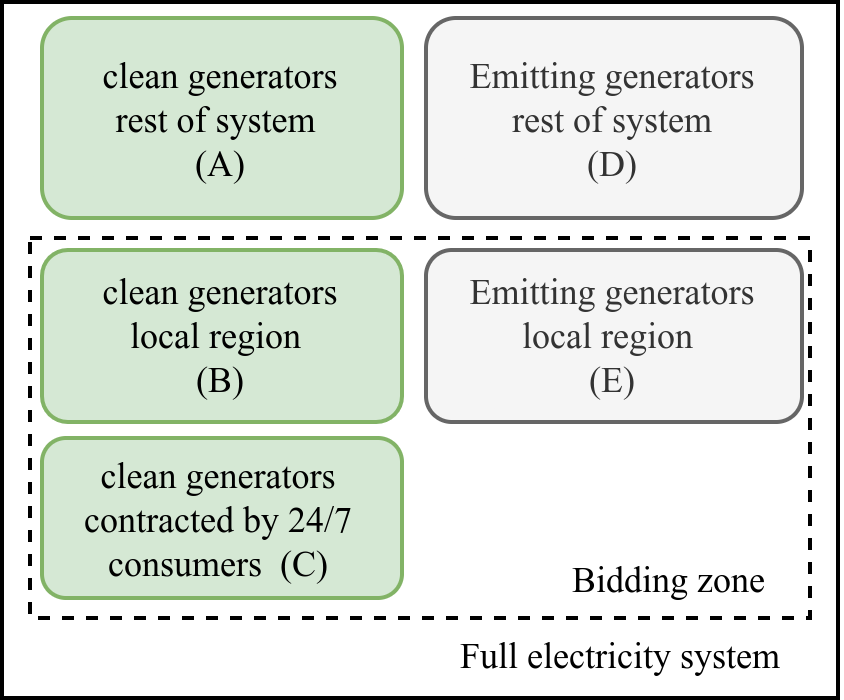
\includegraphics[width=5cm]{images/cfe.png}
  {\scriptsize
  This approach is based on \hrefc{https://acee.princeton.edu/24-7/}{Xu et al. (2021)}
  }
  \end{column}
    
  \end{columns}

  \noindent\fbox{%
  \parbox{\textwidth}{%
  $CFE_t$ can be seen as the percentage of clean electricity in each MWh of imported 
  electricity from the grid to supply participating 24/7 loads in a given hour.
  }}
  }

\end{frame}


\begin{frame}{CO$_2$ emissions rate of the regional grid and 24/7 portfolio, 1/2}

  {\small

  \alert{CO$_2$ emissions} associated with the dispatch of emitting power plants 
  in the European electricity system are part of the model solution.
  We can use this information to calculate (i) the \emph{emissionality} of generation 
  that serves participating 24/7 demand, and (ii) the \emph{avoided emissions}, i.e.,
  the difference in regional CO$_2$ emissions with and without 24/7 procurement. 
  Similarly to the logic of computing the grid CFE factor, 
  we need to consider imported emissions also in this calculation.
  
  First, let $X(D)_t$ be hourly emissions $[tCO_2]$ in the rest of the electricity system. 
  The average emissions rate of the rest of the system is calculated as:

  \begin{equation*}
  SystemEmisRate = \frac{X(D)_t}{A_t + D_t}
  \end{equation*}

  Second, let $Y(E)_t$ be hourly emissions in the regional grid where 24/7 consumers are located.
  The emissions rate of grid supply is then:

  \begin{equation*}
  GridSupplyEmisRate = \frac{Y(E)_t + SystemEmisRate * import_t}{B_t + E_t + import_t}
  \end{equation*}

  }
\end{frame}



\begin{frame}{CO$_2$ emissions rate of the regional grid and 24/7 portfolio, 2/2}

  {\small
  Third, we calculate {CO$_2$ emissions} associated with the electricity consumption of 
  24/7 participating consumers on an hourly basis:
  
  \begin{equation*}
  Emissions_t = GridSupply_t * GridSupplyEmisRate_t
  \end{equation*}

  Now, we have the necessary components to calculate two metrics of interest for our analysis. 
  A first metric is the \alert{average emissions rate of 24/7 consumers}:

  \begin{equation*}
    (C\&I)EmisRate = \frac{\sum_{t\in T} Emissions_t}{\sum_{t\in T} Load_t}
  \end{equation*}

  A second metric is the \alert{avoided emissions} by 24/7 procurement. The calculation is based on the 
  difference between the total {CO$_2$ emissions} in the regional grid where 24/7 consumers are located
  with and without 24/7 procurement (\emph{'247-cfe'} and \emph{'reference'} labels, accordingly):

  \begin{equation*}
    AvoidedEmissions = \sum_{t\in T} Y(E)_t^{reference} - \sum_{t\in T} Y(E)_t^{247-cfe}
  \end{equation*}
  }

\end{frame}


%----------------------------------------
%----------------------------------------
\section{Scenario setup}


\begin{frame}{Scenario setup 1/3}
 
  \begin{columns}[T]
  \begin{column}{7.2cm}

  \centering
  \vspace{0.3cm}
  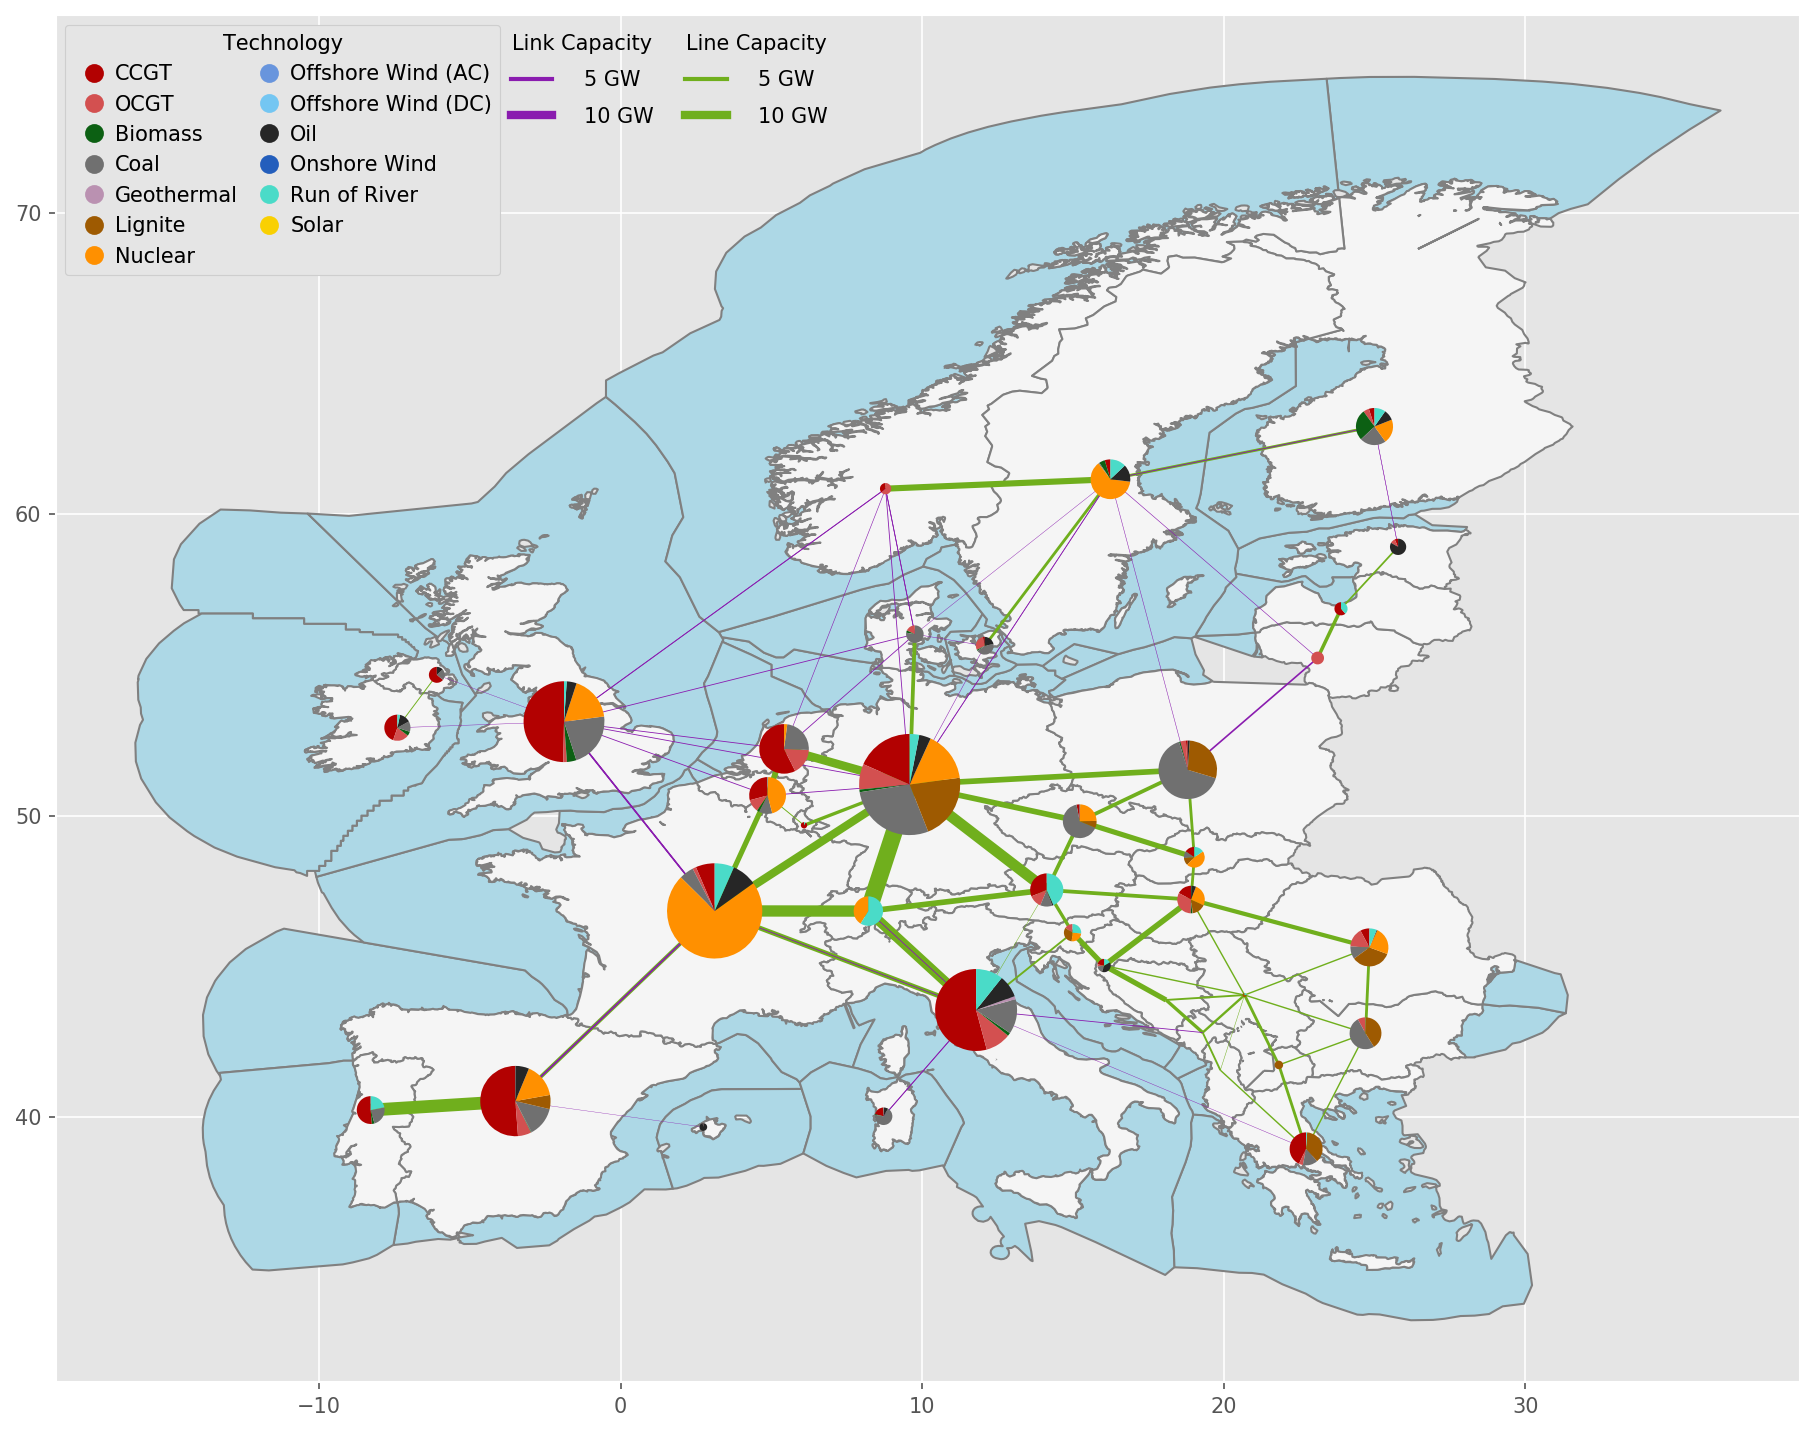
\includegraphics[width=7.5cm]{images/elec_s_37.png}

  {\footnotesize 
  PyPSA-Eur network clustered to 37 zones
  }
  \end{column}

  \begin{column}{8.5cm}
  {\footnotesize 
  \begin{itemize}
  \item In each scenario, we model the full European power system 
  clustered to \alert{37 zones}. 
    
  \item Each zone represents an individual country. Some countries
  that straddle different synchronous areas are split to individual bidding zones, 
  such as DK1 (West) and DK2 (East).

  \item Consumers following 24/7 approach can be located in one of the \alert{four zones}: 
  Ireland, Denmark (zone DK1), Germany and the Netherlands.
    
  \item We assume that all consumers committed to 24/7 matching, form an alliance and sign contracts 
  with CFE generators so that their aggregated consumption can be matched 
  on an hour-by-hour basis with clean generation to achieve a given CFE matching score.\footnote
 {{\scriptsize In reality, C\&I participants can also pursue hourly matching strategies
  independently based on their own specific load profiles. 
  See \hrefc{https://zenodo.org/record/7082212}{Qingyu \& Jenkins (2022)} study investigating this case.}}
  
  \end{itemize}
  }
  
  \end{column}
  \end{columns}

\end{frame}



\begin{frame}{Scenario setup 2/3}

  {\footnotesize 

  We assume that 24/7 consumers have an access to a wide palette
  of carbon-free technologies\footnote{{\scriptsize We consider carbon-free power generation
  technologies that we believe can play important roles in facilitating CFE matching on hourly basis, 
  while enabling deeper decarbonization of electricity systems at the same time. Technology inclusivity is a 
  \hrefc{https://www.gstatic.com/gumdrop/sustainability/24x7-carbon-free-energy-methodologies-metrics.pdf}{principle} 
  of the 24/7 CFE methodology.}} that are either available on the European market now
  or expected to be available for a commercial scale up in the near future. 
  We formulate three scenarios grouping generators by a degree of technological
  maturity as of now:

  \centering
  \begin{table}[h]
  \begin{tabular}{ccc}
    \hline
    \alert{Palette 1} & \alert{Palette 2} &  \alert{Palette 3} \\
    \hline
      onshore wind & onshore wind  & onshore wind \\ 
    \hline
      utility scale solar & utility scale solar  & utility scale solar \\
    \hline
      battery storage & battery storage  & battery storage \\
    \hline
      - & LDES\footnote{{\scriptsize Long-duration energy storage (LDES).}} & LDES \\
    \hline
      - & - & Allam cycle with CCS\footnote{{\scriptsize Allam cycle is a natural gas power plant 
      with up to 100\% of carbon capture and sequestration.}}  \\
    \hline
      - & - & Advanced dispatchable generator\footnote{{\scriptsize A stand-in for clean dispatchable technologies, 
      such as advanced geothermal (closed-loop) or nuclear systems. See e.g., \hrefc{https://www.eavor.com/}{Eavor} 
      developing a promising solution for clean baseload \& dispatchable power with a potential
      for a commercial scale up in Europe.}} \\  
  \end{tabular}
  \end{table}
  }
  \vspace{0.5cm}

\end{frame}



\begin{frame}{Scenario setup 3/3}

  {\footnotesize 
  \begin{itemize}

  \item We model various procurement policies and targets. The scenarios include: \\
  (i) \alert{24/7 CFE matching} with seven different CFE scores in a range from 80\% to 100\%, \\
  (ii) \alert{100\% annual renewable matching} -- the best case scenario for the annual matching policy, \\
  (iii) \alert{A reference case} when 24/7 consumers cover their load purely with grid purchases 
  without any policy regarding the origin of electricity.

  \item We focus on two periods: \alert{2025} and \alert{2030}. The two periods differ by \\ 
  (i) Technology cost assumptions, \\
  (ii) National renewable expansion pathways,\\
  (iii) Power plant fleet (changes take place due to decommissioning based on generators' 
  age or national policies), \\
  (iv) System-wide assumptions, such as price for EU ETS allowances.

  \item We conduct an analysis for different rates of participation. The two scenarios 
  assume that \alert{10\%} and \alert{25\%} of commercial and industrial load
  in a given zone participate in 24/7 CFE matching.

  \item Finally, we conduct an analysis for different (synthetic) load profiles of C\&I participants, which
  represent a \alert{'baseload'} (flat), a \alert{'datacenter'}, and an \alert{'industry consumer'} consumption patterns.   

  \end{itemize}
  }
\end{frame}



%----------------------------------------
%----------------------------------------
\section{Data sources and key assumptions}


\begin{frame}{Summary of data sources: electricity grid}
 
  \begin{columns}[T]
  \begin{column}{7cm}

  \vspace{0.3cm}
  \centering

  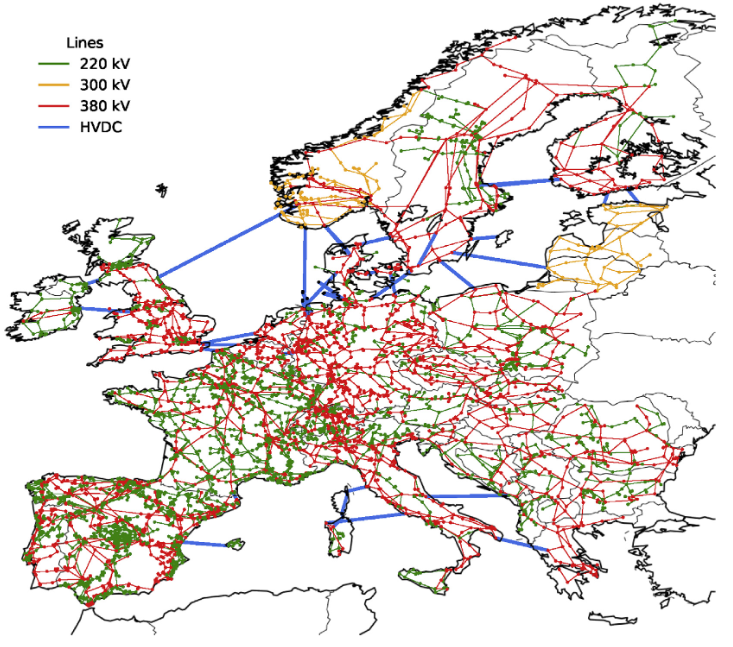
\includegraphics[width=7cm]{images/pypsa-eur-grid.png}

  {\footnotesize 
  \vspace{.1cm}
  Basic validation of grid model in 
  \hrefc{https://doi.org/10.1016/j.esr.2018.08.012}{Hörsch et al. (2018)}
  }
  \end{column}

  \begin{column}{7.5cm}
  {\small 
  \vspace{.3cm}
  \begin{itemize}
    \item Grid data contains AC lines at and above 220~kV voltage level, 
    all high voltage DC lines, and substations for the full 
    \hrefc{https://www.entsoe.eu/data/map/}{ENTSO-E area}.
    \item Grid data is collected by \hrefc{https://github.com/PyPSA/GridKit}{GridKit extraction} 
    of ENTSO-E interactive map
    \item Spatial resolution is
    \hrefc{https://pypsa-eur.readthedocs.io/en/latest/simplification/cluster_network.html}{adjustable}, 
    what allows spatial and topological analysis at different levels 
    (e.g. by transforming the transmission grid to a 380~kV only equivalent network).

  \end{itemize}
  }
  
  \end{column}
  \end{columns}

\end{frame}



\begin{frame}{Summary of data sources: power plants and technology costs}
 
  \begin{columns}[T]\

  \begin{column}{7.5cm}
    {\small 
    \begin{itemize}
      \item Existing generation fleet data is collected by cleaning, 
      standardizing and merging multiple power plant databases.
      
      \item The process is transparent and open-sourced via the 
      \hrefc{https://github.com/PyPSA/powerplantmatching}{powerplantmatching} package.
      The package provides all the important information about power plants in a ready-to-use format
      for the European power system. 
  
      \item Assumptions on energy system technologies (such as capital and operational costs, efficiencies, lifetimes, etc.) 
      are gathered from variety of open sources. The process is also open-sourced via the 
      \hrefc{https://github.com/PyPSA/technology-data}{technology-data} project. 
  
      \item Both tools are maintained by TU Berlin team.
  
    \end{itemize}
    }  
  \end{column}

  \begin{column}{7cm}

  \vspace{0.3cm}
  \centering

  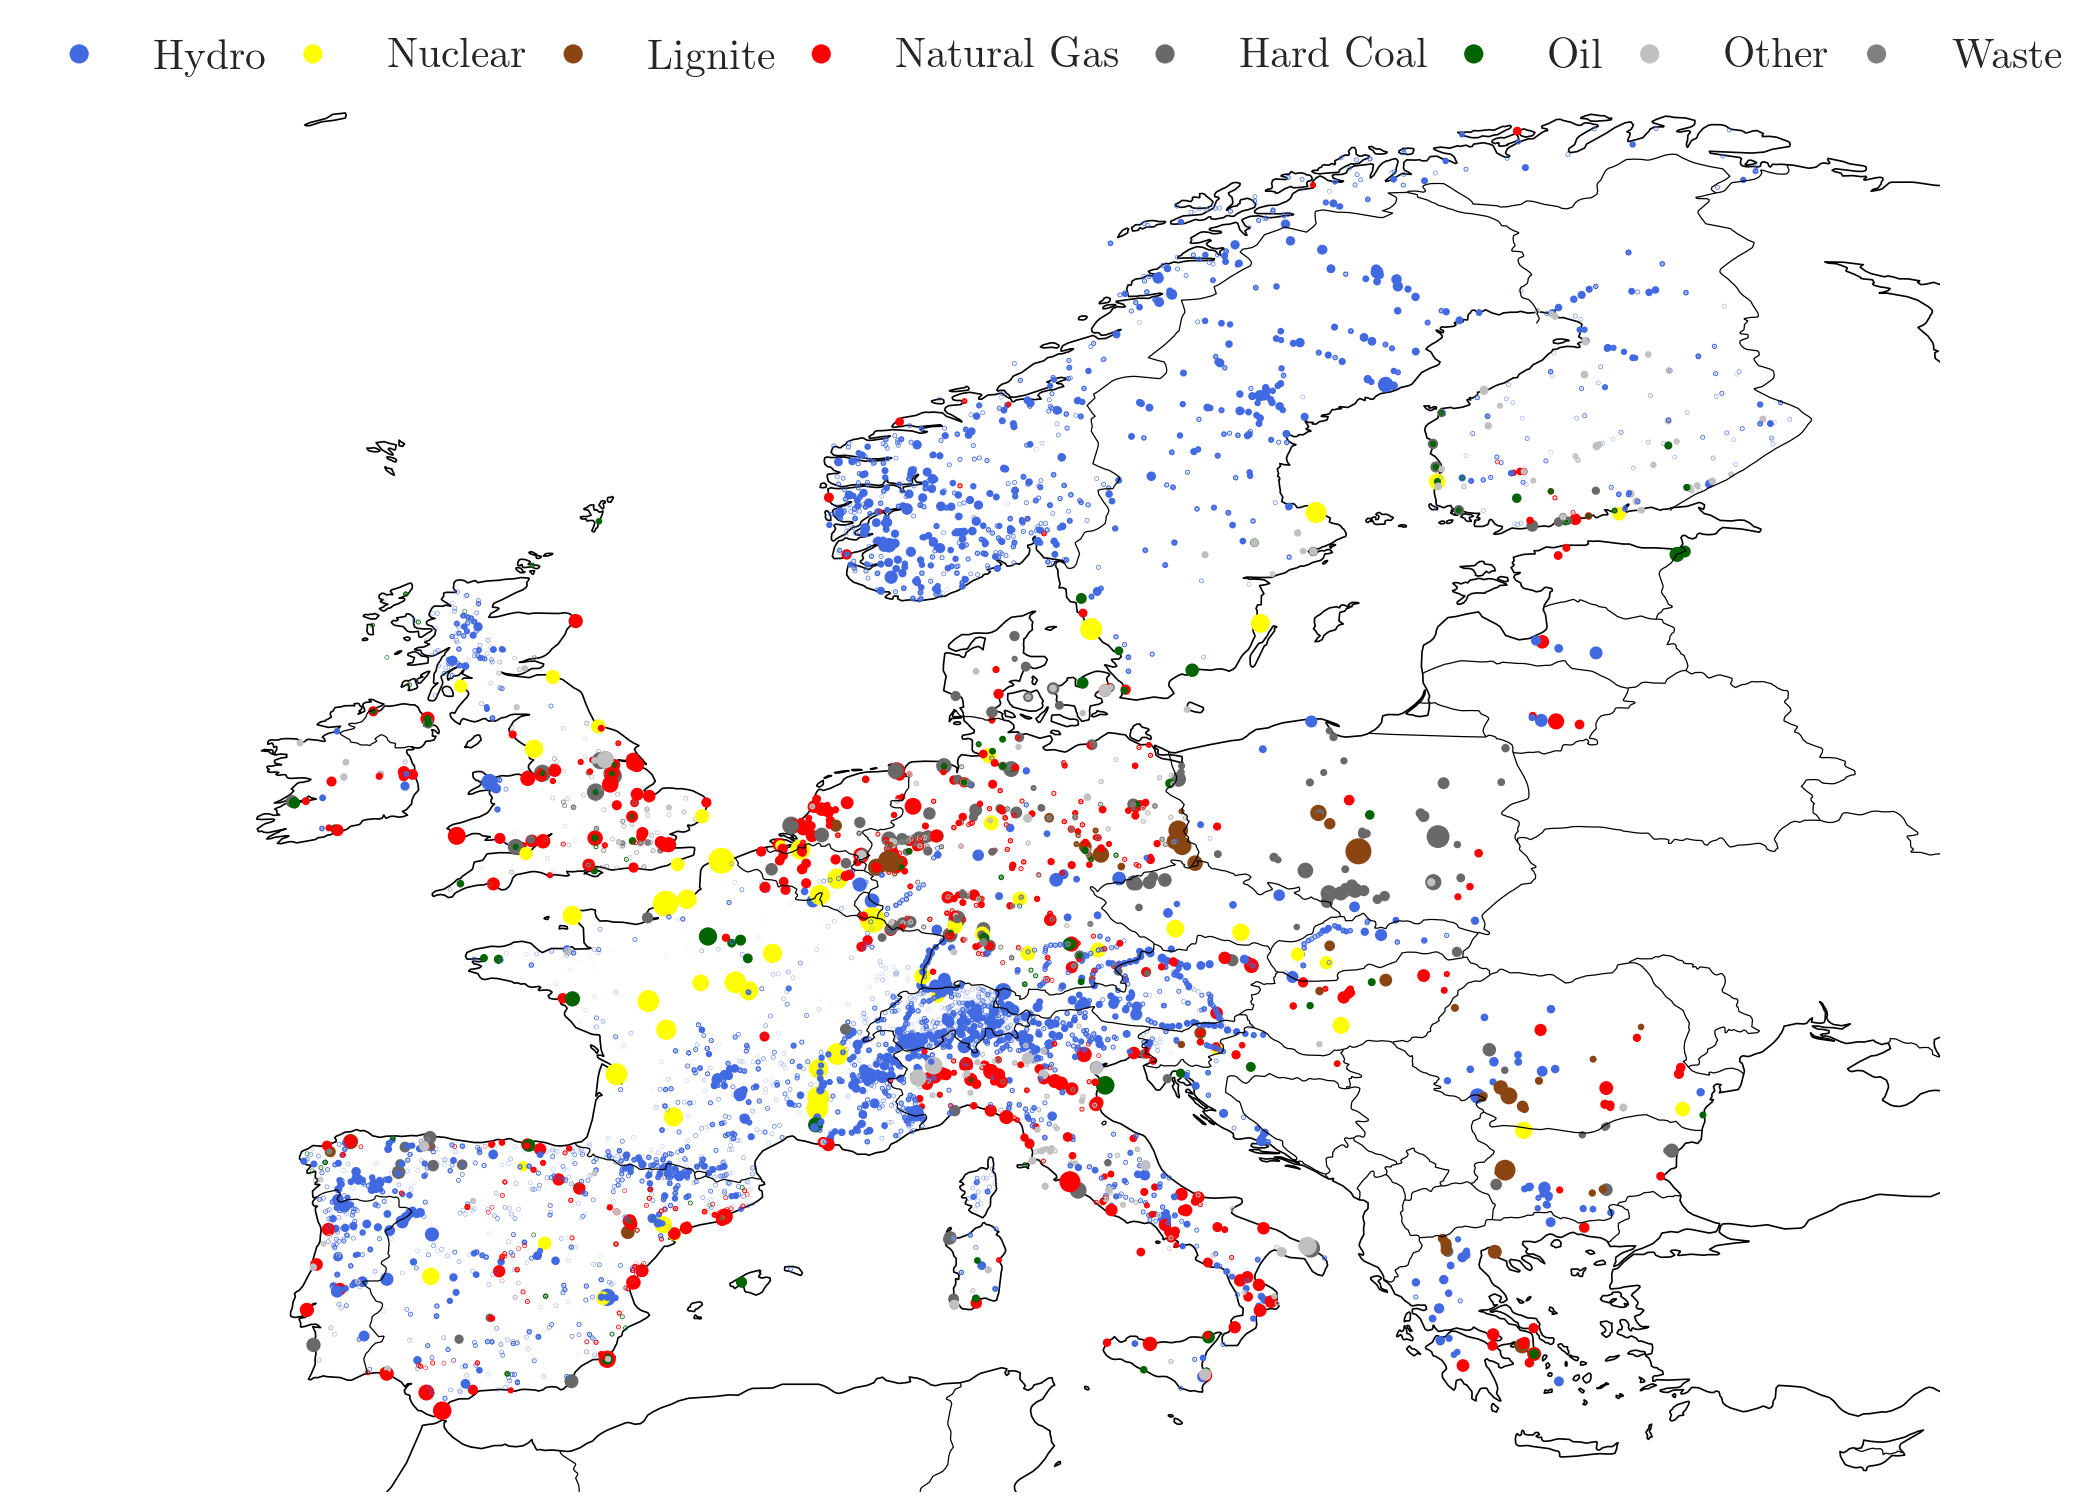
\includegraphics[width=7cm]{images/powerplantmatching.png}

  {\footnotesize 
  \vspace{0.1cm}
  A showcase example 
  of \hrefc{https://github.com/PyPSA/powerplantmatching}{powerplantmatching}
  }
  \end{column}
  \end{columns}

\end{frame}



\begin{frame}{Summary of data sources: renewable potentials and time series}
 
  \begin{columns}[T]
  \begin{column}{9cm}

  \vspace{0.3cm}
  \centering

  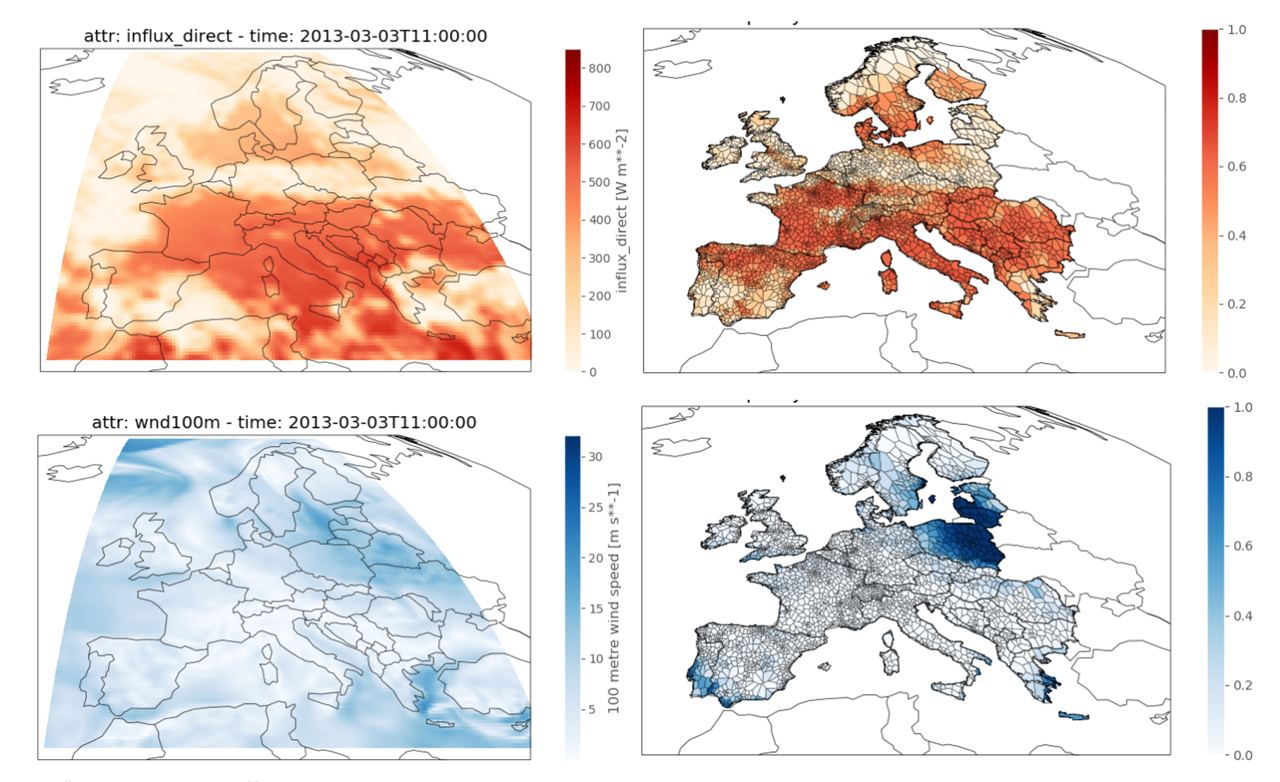
\includegraphics[width=9cm]{images/atlite.jpg}

  {\footnotesize 
  Converting weather data to energy system data with \hrefc{https://github.com/PyPSA/atlite}{atlite}
  }
  \end{column}

  \begin{column}{7cm}
  {\small 
  \begin{itemize}
    \item Renewable power potentials and generation profiles are processed by 
    the open-source \hrefc{https://github.com/PyPSA/atlite}{atlite} package, 
    which converts terabytes of weather data (like wind speeds, solar influx) 
    into the data for energy systems modelling.
    \item Geographic potentials for renewable energy are based on the
    \hrefc{https://github.com/FZJ-IEK3-VSA/glaes}{GLAES} framework. We gather and process
    datasets for land cover (CORINE2018), natural protection areas (NATURA2000),
    bathymetry (GEBCO2018) and \hrefc{https://pypsa-eur.readthedocs.io/en/latest/}{other} 
    to conduct own geospatial land availability analysis.
    \item The \alert{atlite} project is also maintained by TU Berlin team.

  \end{itemize}
  }
  
  \end{column}
  \end{columns}

\end{frame}


\begin{frame}{Other assumptions}

\begin{itemize}
  {\small 
\item Model is set to perform a \alert{perfect-foresight optimization} of investment 
and power dispatch decisions to meet electricity demand of the 24/7 consumers, 
as well as the demand of other consumers in the European electricity system for 2025 or 2030.
\item Electrical demand time-series is based on the 
\hrefc{https://open-power-system-data.org/}{OPSD project}. 
We assume the same demand profile per bidding zone for 2025 and 2030, as in the representative year 2013.
\item Similarly, we assume 2013 as the representative climate year for renewable in-feed.
\item Renewable expansion in the regional grid where 24/7 consumers are located is based on the 
\hrefc{https://energy.ec.europa.eu/topics/energy-strategy/national-energy-and-climate-plans-necps_en}{national energy and climate plans}.\footnote{{\scriptsize For Germany, we assume the 
\hrefc{https://www.bmwk.de/Redaktion/EN/Pressemitteilungen/2022/04/20220406-federal-minister-robert-habeck-says-easter-package-is-accelerator-for-renewable-energy.html}{Easter package}
to come into force as planned, i.e. RES cover 80\% of gross electricity consumption by 2030.}}
\item  National policies and decommissioning plans for coal and nuclear 
power plants are based on the 
\hrefc{https://beyond-coal.eu/}{Europe Beyond Coal}, 
and \hrefc{https://world-nuclear.org/}{world-nuclear.org} projects.
\item We assume price for EU ETS allowances to be 80~\euro/tCO$_2$ 
and 130~\euro/tCO$_2$ for 2025 and 2030, accordingly. The price for 
natural gas is assumed to be 35~\euro/MWh.\footnote{{\scriptsize Based on the price assumptions in the \hrefc{https://energy.ec.europa.eu/system/files/2022-05/SWD_2022_230_1_EN_autre_document_travail_service_part1_v3.pdf}{REPowerEU Plan}
issued by the European Commission in May 2022}}
}
\vspace{0.2cm}
\end{itemize}

\end{frame}


\begin{frame}{Technologies available for 24/7 consumers - 2025}
  
  {\scriptsize 

    \begin{tabular}{cccccccc}
      \hline
      Palette & Technology & CAPEX & FOM & VOM & Eff. & lifetime & Original reference \\
       &  & (overnight cost)  &  (\%/year) &  (€/MWh) & (per unit) & (years) & (\hrefc{https://github.com/PyPSA/technology-data}{technology data}) \\
      \hline
      1,2,3 & solar & 612 €/kW & 1.7 & 0.01 & - & 37.5 & \hrefc{https://ens.dk/en/our-services/projections-and-models/technology-data}{DEA}\\
      \hline
      1,2,3 & onshore wind & 1077 €/kW & 1.2 & 1.42 & - & 28.5 & \hrefc{https://ens.dk/en/our-services/projections-and-models/technology-data}{DEA}\\
      \hline
      1,2,3 & battery storage & 187 €/kWh & - & - & - & 22.5 & \hrefc{https://ens.dk/en/our-services/projections-and-models/technology-data}{DEA} \\
      \hline
      1,2,3  & battery inverter & 215 €/kW & 0.3 & - & 0.96  & 10.0 & \hrefc{https://ens.dk/en/our-services/projections-and-models/technology-data}{DEA} \\
      \hline
      2,3 & hydrogen storage\footnote{{\scriptsize Underground hydrogen storage in salt cavern}} 
                  & 2.5 €/kWh & 0 & 0 & - & 100.0 & \hrefc{https://ens.dk/en/our-services/projections-and-models/technology-data}{DEA} \\
      \hline
      2,3 & electrolysis & 550 €/kW & 2.0 & - & 0.67 & 27.5 & \hrefc{https://ens.dk/en/our-services/projections-and-models/technology-data}{DEA} \\
      \hline
      2,3 & fuel cell & 1200 €/kW & 5.0 & - & 0.50 & 10.0 & \hrefc{https://ens.dk/en/our-services/projections-and-models/technology-data}{DEA} \\
      \hline
      3 & NG Allam cycle\footnote{{\scriptsize Costs also include estimate of 40~€/ton for CO$_2$ transport \& sequestration.}} & 2760 €/kW & 14.8  & 3.2 & 0.54 & 30.0 &
      \hrefc{https://file.go.gov.sg/carbon-capture-utilisation-and-storage-decarbonisation-pathway-for-singapore-energy-and-chemical-sectors-pdf.pdf}{Navigant}, 
      \hrefc{https://netzeroamerica.princeton.edu/}{NZA}\\
      \hline
      3 & Advanced dispatchable
      & 10000 €/kW & 0 & 0 & 1.00 & 30.0 & own assumption \\
      \end{tabular}
  }

\end{frame}



\begin{frame}{Technologies available for 24/7 consumers - 2030}
  
  {\scriptsize 

    \begin{tabular}{cccccccc}
      \hline
      Palette & Technology & CAPEX & FOM & VOM & Eff. & lifetime & Original reference \\
       &  & (overnight cost)  &  (\%/year) &  (€/MWh) & (per unit) & (years) & (\hrefc{https://github.com/PyPSA/technology-data}{technology data}) \\
      \hline
      1,2,3 & solar & 492 €/kW & 2.0 & 0.01 & - & 40 & \hrefc{https://ens.dk/en/our-services/projections-and-models/technology-data}{DEA}\\
      \hline
      1,2,3 & onshore wind & 1035 €/kW & 1.2 & 1.35 & - & 30 & \hrefc{https://ens.dk/en/our-services/projections-and-models/technology-data}{DEA}\\
      \hline
      1,2,3 & battery storage & 142 €/kWh & - & - & - & 25.0 & \hrefc{https://ens.dk/en/our-services/projections-and-models/technology-data}{DEA} \\
      \hline
      1,2,3  & battery inverter & 160 €/kW & 0.3 & - & 0.96  & 10.0 & \hrefc{https://ens.dk/en/our-services/projections-and-models/technology-data}{DEA} \\
      \hline
      2,3 & hydrogen storage\footnote{{\scriptsize Underground hydrogen storage in salt cavern}} 
                  & 2.0 €/kWh & 0 & 0 & - & 100 & \hrefc{https://ens.dk/en/our-services/projections-and-models/technology-data}{DEA} \\
      \hline
      2,3 & electrolysis & 450 €/kW & 2.0 & - & 0.68 & 30.0 & \hrefc{https://ens.dk/en/our-services/projections-and-models/technology-data}{DEA} \\
      \hline
      2,3 & fuel cell & 1100 €/kW & 5.0 & - & 0.5 & 10.0 & \hrefc{https://ens.dk/en/our-services/projections-and-models/technology-data}{DEA} \\
      \hline
      3 & NG Allam cycle\footnote{{\scriptsize Costs also include estimate of 40~€/ton for CO$_2$ transport \& sequestration.}}  & 2600 €/kW & 14.8  & 3.2 & 0.54 & 30 &
      \hrefc{https://file.go.gov.sg/carbon-capture-utilisation-and-storage-decarbonisation-pathway-for-singapore-energy-and-chemical-sectors-pdf.pdf}{Navigant}, 
      \hrefc{https://netzeroamerica.princeton.edu/}{NZA}\\
      \hline
      3& Advanced dispatchable
      & 10000 €/kW & 0 & 0 & 1 & 30 & own assumption \\
      \end{tabular}
  }

\end{frame}


%---------------------------------------------
%---------------------------------------------
\section{Modelling results and analysis}


%----------------------------------

\begin{frame}{Scenario space}

  {\small
  The following section presents modelling results and related analysis. 
  For convenience, we start with a \alert{base scenario} 
  with the following setup:

    \quad{\bf Zone:} IE | DE | DK1 | NL \\
    \quad{\bf Technology palette:} 1 | 2 | 3 \\
    \quad{\bf Year:} 2025 \\ 
    \quad{\bf Participation rate:} 10\% of C\&I demand in a modelled zone \\
    \quad{\bf Demand profile}: baseload (flat) \\
  
  \vspace{0.3cm}
  Afterwards, we explore the scenario space further by implementing one-at-a-time 
  adjustments to the base scenario: \\
  (i) implementing year {\bf 2030}, \\
  (ii) implementing participation rate of {\bf 25\%}, \\ 
  (iii) implementing {\bf other types of demand profiles} for C\&I consumers.
  
  \vspace{0.3cm}
  For interested parties, we publish an \hrefc{https://doi.org/10.5281/zenodo.7180098}{online annex} 
  with a full pack of modelling results alongside this study. The annex 
  includes modelling results for all scenario combinations.
  }
  \end{frame}

%----------------------------------

\begin{frame}{Base scenario: Ireland -- Palette 1}

{\footnotesize
\vspace{0.3cm}

\begin{columns}[T]
\begin{column}{9cm}
\centering

\includegraphics[width=9.4cm]{../results/report/plots/10/2025/IE/p1/used.pdf}
\end{column}
\begin{column}{6cm}

\vspace{0.1cm}
A plot on the left shows the {\bf fraction of hourly demand met with carbon-free
electricity} depending on the procurement policy that C\&I consumers follow.

\vspace{0.3cm}
In the reference case, where C\&I consumers do not procure any resources,  
relying purely on grid purchases, \alert{only 61\%} of demand is met with CFE.

\vspace{0.3cm}
100\% RES -- the best case for the annual renewable matching policy -- 
results in 85\% fraction. Thus, \alert{CFE targets beyond 85\%} yield 
higher share of hourly demand met with CFE
than 100\% RES procurement policy.

\vspace{0.3cm}
When CFE target approaches 100\%, C\&I participants 
\alert{rely more on procured resources}.

\end{column}
\end{columns}
}
\source{Ireland -- Palette 1 -- 2025 -- 10\% -- baseload}
\end{frame}



\begin{frame}{Base scenario: Ireland -- Palette 1}

{\footnotesize
\vspace{0.3cm}

\begin{columns}[T]
\begin{column}{9cm}
\centering

\includegraphics[width=9.4cm]{../results/report/plots/10/2025/IE/p1/ci_emisrate.pdf}

\end{column}
\begin{column}{6cm}

\vspace{0.1cm}
Next, we investigate how the choice of a procurement policy affects the {\bf average emissions 
rate} of 24/7 participating C\&I consumers.

\vspace{0.3cm}
Already in 2025, Ireland has a moderately clean electricity system: 
the C\&I emission rate in the reference case is at 138~kg/MWh.

\vspace{0.3cm}
100\% annual matching with renewable energy reduces the 
C\&I emission rate to 53 kg/MWh.

\vspace{0.3cm}
When actively matching the carbon-free electricity and the load with 
24/7 procurement, C\&I participants can achieve \alert{lower emission 
rates than with the 100\% RES policy} with CFE targets beyond 85\%. 
As CFE target is tightened further, average emissions \alert{drop to zero}.

\end{column}
\end{columns}
}
\source{Ireland -- Palette 1 -- 2025 -- 10\% -- baseload}
\end{frame}



\begin{frame}{Base scenario: Ireland -- Palette 1}

  {\footnotesize
  \vspace{0.3cm}
  
  \begin{columns}[T]
  \begin{column}{9cm}
  \centering
  
  \includegraphics[width=9.4cm]{../results/report/plots/10/2025/IE/p1/ci_capacity.pdf}
  \end{column}
  \begin{column}{6cm}
  
  \vspace{0.1cm}
  If we now turn to the {\bf portfolio capacity} procured by 
  C\&I consumers, we see that at this level of participation
  (10\% of C\&I load in Ireland is at 220~MW), the 100\% RES policy can be 
  me by procuring near to 1.5~GW of onshore wind and solar generators.
  
  \vspace{0.3cm}
  In this scenario, hourly matching renewable generation and the 24/7 participating load
  requires a \alert{much bigger portfolio} of renewable generators than the 
  100\% RES policy. 

  \vspace{0.3cm}
  Also, above 85\% 24/7 procurement sees \alert{battery storage} enter the portfolio  mix.
  
  \vspace{0.3cm}
  Note that for 80\% CFE, 24/7 participating C\&I consumers procure less 
  capacity than for 100\% RES policy, as it relies more on grid imports.

  \end{column}
  \end{columns}
  }
  \source{Ireland -- Palette 1 -- 2025 -- 10\% -- baseload}
  \end{frame}



\begin{frame}{Base scenario: Ireland -- Palette 1}

    {\footnotesize
    \vspace{0.3cm}
    
    \begin{columns}[T]
    \begin{column}{9cm}
    \centering
    
    \includegraphics[width=9.4cm]{../results/report/plots/10/2025/IE/p1/ci_costandrev.pdf}
    \end{column}
    \begin{column}{6cm}
    
    \vspace{0.1cm}
    It is also interesting to look at the {\bf breakdown of costs associated with
    a procurement policy} that C\&I consumers choose. 
    
    \vspace{0.3cm}
    Note that revenues from selling the excess electricity to the regional grid 
    (dark green) at market prices can be treated as "negative costs" and 
    subtracted from the net procurement cost.

    \vspace{0.3cm}
    A CFE target of 90-95\% can be achieved at a small cost premium to 100\% 
    annual renewable matching with solar, wind and batteries. However,
    what stands out in the plot is the rapid increase of procurement costs  
    for high CFE targets. For example, 98\% CFE target has 
    cost premium of only 55\% over 100\% annual renewable matching; while
    \alert{the last 2\% of hourly CFE matching more than doubles the 
    cost}.
  
    \end{column}
    \end{columns}
    }
    \source{Ireland -- Palette 1 -- 2025 -- 10\% -- baseload}
    \end{frame}



\begin{frame}{Base scenario: Ireland -- Palette 2}

    {\footnotesize
  
    \begin{columns}
    \begin{column}{7cm}
    \centering
    \includegraphics[width=7.5cm]{../results/report/plots/10/2025/IE/p2/ci_capacity.pdf}
    \end{column}
  
    \begin{column}{8cm}
    \centering
    \includegraphics[width=7.5cm]{../results/report/plots/10/2025/IE/p2/ci_costandrev.pdf}
    \end{column}
  
    \end{columns}
  
    \begin{columns}
    \begin{column}{15cm}
    If we look at the results for the technological {\bf Palette 2} -- 
    when C\&I consumers have an access to the long-duration energy storage (LDES) --
    we see a different picture. The portfolio of renewable capacity 
    C\&I consumers for the 100\% CFE target is not much larger 
    than for 100\% RES (see the left panel). The LDES system helps to align the load 
    with the generation of procured variable renewable resources. 
    In the right panel, we can see that a LDES system (here 2.5~€/kWh 
    hydrogen storage in caverns) can \alert{significantly limit the procurement cost
    increase} at high CFE targets. In this scenario, 
    100\% CFE costs only 50\% more than a 100\% RES policy.

    \end{column}
    \end{columns}
    }
  
    \source{Ireland -- Palette 2 -- 2025 -- 10\% -- baseload}
\end{frame}



\begin{frame}{Base scenario: Ireland -- Palette 3}

  {\footnotesize

  \begin{columns}
  \begin{column}{7cm}
  \centering
  \includegraphics[width=7.5cm]{../results/report/plots/10/2025/IE/p3/ci_capacity.pdf}
  \end{column}

  \begin{column}{8cm}
  \centering
  \includegraphics[width=7.5cm]{../results/report/plots/10/2025/IE/p3/ci_costandrev.pdf}
  \end{column}

  \end{columns}

  \begin{columns}
  \begin{column}{15cm}
  Finally, the results for technological {\bf Palette 3} scenario show that 24/7 procurement
  can create a market for and benefit from the advanced technologies such as 
  NG Allam Cycle generator with carbon capture and sequestration or 
  advanced geothermal systems. 
  In the case of Ireland, NG Allam Cycle generator is added to the 
  procured portfolio. The clean dispatchable technology \alert{further limits 
  the hourly CFE cost premium} above annual renewable matching. 
  Inclusion of clean firm generation also reduces storage requirements.
  \end{column}
  \end{columns}
  }

  \source{Ireland -- Palette 3 -- 2025 -- 10\% -- baseload}
\end{frame}

%----- base scenario, system effects


\begin{frame}{Base scenario: Ireland -- Palette 3}

  {\footnotesize
  \vspace{0.1cm}
  
  \begin{columns}[T]
  \begin{column}{9cm}
  \centering
  
  \includegraphics[width=9.4cm]{../results/report/plots/10/2025/IE/p3/zone_emissions.pdf}
  
  \end{column}
  \begin{column}{6cm}
  
  \vspace{0.1cm}
  In the next step, we explore how the 24/7 procurement affects the 
  rest of the electricity system. The plot on the left shows
  {\bf CO$_2$~emissions in the local region} of 24/7 participating 
  consumers -- Ireland.
  
  \vspace{0.1cm}
  Without any procurement, the model estimates 
  Irish power sector carbon emissions to be at the level of 3.5~MtCO$_2$
  (for comparison, 
  \hrefc{https://www.seai.ie/data-and-insights/seai-statistics/key-statistics/co2/}{seai.ie}
  reports this value to be at 8.4~MtCO$_2$ in 2020, with a strong decreasing trend).

  \vspace{0.1cm}
  100\% annual renewable matching can deliver greater system-level CO$_2$ emissions
  reductions than lower CFE scores. 100\% RES reduces emissions in Ireland by 
  ca. 0.6~MtCO$_2$ per year (at 10\% participation rate).
  
  \vspace{0.1cm}
  However, beyond 85\% CFE targets, 24/7 hourly matching achieves
  \alert{greater emissions reductions} than 100\% RES.

  \end{column}
  \end{columns}
  }
  \source{Ireland -- Palette 3 -- 2025 -- 10\% -- baseload}
\end{frame}

%----------------------------------------
%Base scenario - other countries

\begin{frame}{Base scenario: other regions}
  \centering
  
  Results for other regions in Europe where C\&I load commits to voluntary  \\ 
  CFE procurement 
  show \alert{similar trends.} \\ 
  
  \vspace{0.3cm}
  However, each region has a \alert{unique set of characteristics} 
  that depend on local resources, renewable potentials,
  national energy and climate policies, degree of interconnections, etc.

  \vspace{0.3cm}
  Despite regional differences, the dynamics of 24/7 CFE procurement, \\
  observed in the example of Ireland, repeat in other regions.

\end{frame}

%----------------------------------------

\begin{frame}{Base scenario: Germany -- Palette 1}

  {\footnotesize
  \vspace{0.1cm}
  
  \begin{columns}[T]
  \begin{column}{9cm}
  \centering
  
  \includegraphics[width=9.4cm]{../results/report/plots/10/2025/DE/p1/used.pdf}
  \end{column}
  \begin{column}{6cm}
  
  \vspace{0.1cm}
  In comparison to the case of Ireland, the German grid is cleaner in 2025, 
  in particular due to good interconnections with e.g., France and Denmark. 
  Thus, without procuring any resources, C\&I consumers reach
  a 79\% share of demand met with CFE.
 
  \vspace{0.3cm}
  The cleaner grid results in a higher fraction (ca. 92\% CFE)
  achieved with the 100\% annual renewable matching policy. 
  
  \vspace{0.3cm}
  Similar to the Irish results, C\&I participants rely more on procured 
  resources with tighter CFE targets.

  \vspace{0.3cm}
  Note that for lower CFE targets, constraint (\ref{eqn:CFE}) 
  is not binding, what makes the same cost-optimal shares of 
  procured portfolio and grid imports repeat
  until the CFE target becomes tight enough.
  
  \end{column}
  \end{columns}
  }
  \source{Germany -- Palette 1 -- 2025 -- 10\% -- baseload}
  \end{frame}
  
  
  
  \begin{frame}{Base scenario: Germany -- Palette 1}
  
  {\footnotesize
  \vspace{0.3cm}
  
  \begin{columns}[T]
  \begin{column}{9cm}
  \centering
  
  \includegraphics[width=9.4cm]{../results/report/plots/10/2025/DE/p1/ci_emisrate.pdf}
  
  \end{column}
  \begin{column}{6cm}
  
  \vspace{0.1cm}
  As can be expected, the cleaner grid in the German case results in 
  a lower value of the average emissions rate of 24/7 participating 
  C\&I consumers than in the case of Ireland. The value is at 92~kg/MWh 
  in the reference case.
  
  \vspace{0.3cm}
  As in Ireland, \alert{two key observations} can be made: \\ 

  \vspace{0.1cm}
  (i) the voluntary commitment to 100\% annual matching 
  with renewable energy greatly reduces the C\&I emission rate, to 34~kg/MWh
  in this case, and \\
  \vspace{0.1cm}
  (ii) with 24/7 CFE procurement, C\&I participants achieve much lower emissions 
  rates than 100\% annual matching with higher CFE targets. Emissions rates 
  fall to zero at 100\% CFE score.

  \end{column}
  \end{columns}
  }
  \source{Germany -- Palette 1 -- 2025 -- 10\% -- baseload}
  \end{frame}
  


\begin{frame}{Base scenario: Germany -- Palette 3}

    {\footnotesize
  
    \begin{columns}
    \begin{column}{7cm}
    \centering
    \includegraphics[width=7.5cm]{../results/report/plots/10/2025/DE/p3/ci_capacity.pdf}
    \end{column}
  
    \begin{column}{8cm}
    \centering
    \includegraphics[width=7.5cm]{../results/report/plots/10/2025/DE/p3/ci_costandrev.pdf}
    \end{column}
  
    \end{columns}
  
    \begin{columns}
    \begin{column}{15cm}
     
    What stands out in the results for Germany is the cost-optimal 
    portfolio procured by C\&I consumers. 
    The plots on top show the porfolio capacity and the procurement 
    costs for one selected technology scenario -- {\bf Palette 3}.
    In this case, the 24/7 CFE requires
    \alert{considerably less renewable capacity} in the portfolio 
    compared to 100\% RES. The reason for this is two-fold. 
    To achieve lower CFE targets, C\&I consumers can complement portfolio with larger volume of 
    imports from the fairly clean grid. 
    To achieve higher CFE targets, an \alert{advanced dispatchable generator}
    is added to the C\&I portfolio that greatly reduces the need 
    for renewable energy to match load on an hourly basis.
    \end{column}
    \end{columns}
    }
  
    \source{Germany -- Palette 3 -- 2025 -- 10\% -- baseload}
  \end{frame}



\begin{frame}{Base scenario: Germany -- Palette 3}

  {\footnotesize
  \vspace{0.1cm}
  
  \begin{columns}[T]
  \begin{column}{9cm}
  \centering
  
  \includegraphics[width=9.4cm]{../results/report/plots/10/2025/DE/p3/zone_emissions.pdf}
  
  \end{column}
  \begin{column}{6cm}
  
  \vspace{0.1cm}
  Another result that stands out in the case of Germany is the
  impact of the 24/7 procurement on the system-level CO$_2$~emissions. 
  
  \vspace{0.1cm}
  Without any CFE procurement stategy, 
  the German power sector carbon emissions are at the level of 
  40.6~MtCO$_2$ in 2025.
  
  \vspace{0.1cm}
  With just 10\% participation rate, ca. \alert{3.8~GW} of C\&I load 
  follows voluntary procurement. 
  With this participation, the 100\% RES can reduce system-level 
  CO$_2$ emissions by \alert{6~MtCO$_2$} per year.
  With the 24/7 hourly matching, C\&I consumers  
  achieve greater impact on emissions, up to \alert{8~MtCO$_2$} per year
  with CFE 100\% target.

  \vspace{0.1cm}
  NB this impact can be achieved with just a \alert{10\% cost premium}
  on top of the 100\% annual renewable matching (see C\&I cost analysis above).

  \end{column}
  \end{columns}
  }
  \source{Germany -- Palette 3 -- 2025 -- 10\% -- baseload}
\end{frame}


\begin{frame}{Base scenario: summary of costs for 24/7 participating consumers}

  {\small 

  Net procurement costs of achieving 98\% and 100\% CFE targets
  (and \% increase compared to the 100\% annual renewable matching) 
  for the base scenario (2020~\euro/MWh):
  }
  \begin{columns}[T]
  \begin{column}{5cm}
   \centering
    \vspace{0.4cm}
    \noindent\fbox{%
    \parbox{\textwidth}{%
    {\footnotesize
    High CFE targets could have a \alert{much smaller cost premium} if long duration storage or 
      clean dispatchable technologies like advanced geothermal are available.
    }}}

    \vspace{0.3cm}
    \noindent\fbox{%
    \parbox{\textwidth}{%
    {\footnotesize
    NB: This calculation assumes that the costs of 24/7 procurement 
    are internalized by participants; i.e., C\&I participants are responsible 
    for paying 100\% of the incremental system costs resulting from 24/7 
    procurement.
    }}}
    
  \end{column}

  \begin{column}{9cm}
  
  \centering
  {\footnotesize
  \begin{table}[h]
  \begin{tabular}{ccccc}
    \hline
    {\bf Zone} & {\bf Palette} &  {\bf 100\% RES} & {\bf 98\% CFE} & {\bf 100\% CFE} \\
    \hline
    \hline
    IE & Palette 1 & 67.1 & 104.2(+55\%) & 229.4(+242\%) \\ 
    \hline
    IE & Palette 2 & 67.1 & 84.6(+26\%) & 98.6(+47\%) \\
    \hline
    IE & Palette 3 & 67.1 & 81.0(+21\%) & 88.1(+31\%) \\
    \hline
    \hline
    DE & Palette 1 & 80.5 & 98.3(+22\%) & 193.5(+141\%) \\ 
    \hline
    DE & Palette 2 & 80.5 & 92.2(+15\%) & 113.5(+41\%) \\
    \hline
    DE & Palette 3 & 80.5 & 82.9(+3\%) & 88.6(+10\%) \\
    \hline
    \hline
    DK1 & Palette 1 & 56.0 & 70.3(+26\%) & 153.7(+175\%) \\ 
    \hline
    DK1  & Palette 2 & 56.0 & 65.2(+16\%) & 84.7(+51\%) \\
    \hline
    DK1  &  Palette 3 & 56.0 & 62.7(+12\%) & 77.1(+38\%) \\
    \hline
    \hline
    NL & Palette 1 & 63.7 & 91.1(+43\%) & 172.1(+170\%) \\ 
    \hline
    NL & Palette 2 & 63.7 & 78.6(+23\%)  & 92.2(+45\%) \\
    \hline
    NL &  Palette 3 & 63.7 & 73.5(+15\%) & 82.5(+29\%) \\
  \end{tabular}
  \end{table}
  }

\end{column}
\end{columns}
\end{frame}




%----------------------------------------
%The effects of moving to 2030

\begin{frame}{The effects of moving to 2030}
  \centering
  
  So far, we have been exploring 24/7 CFE procurement \\ 
  within the European electricity system in {\bf 2025}. \\ 
  
  \vspace{0.3cm}
  However, what happens if we look 5 years more ahead -- in \alert{2030}? 

  \vspace{1cm}
  \noindent\fbox{%
  \parbox{\textwidth}{%
  {\small
  From the modelling perspective, {\bf many system parameters change} 
  with a step to 2030. In particular, the technology costs decline 
  due to economics of scale and incremental innovation, national 
  energy- and climate policies become more tight, some legacy power plants leave the market. An overarching feature of the energy transition is
  a \alert{cleaner state of the electricity grids}.
  }}}

\end{frame}


%----------------------------------------
%2030
 
\begin{frame}{2030 scenario: Ireland -- Palette 3}

{\footnotesize

\begin{columns}[T]
\begin{column}{9cm}
\centering

\includegraphics[width=9.4cm]{../results/report/plots/10/2030/IE/p3/used.pdf}
\end{column}
\begin{column}{6cm}

\vspace{0.1cm}
The plot on the left shows {\bf the fraction of hourly demand met with CFE} 
for different procurement policies for C\&I load in Ireland -- now for 2030.
The first observation is that in the reference case,
74\% of demand is met with CFE, which is 13\% more than in 2025. 
Furthermore, there are \alert{two findings} 
on the hourly 24/7 matching: \\

\vspace{0.1cm}
{\bf First}, lower CFE targets (such as 80\%) can be met without 
any procurement of renewable generators by C\&I consumers. Instead,
the target is reached by a combination of grid imports and battery
storage (see next slide). \\

\vspace{0.1cm}
{\bf Second}, grid imports can still play a role in reaching 100\% CFE,
as LDES and advanced dispatchable technologies offer flexibility
in matching renewable generation with C\&I load on hourly basis, while 
grid imports are possible during the hours when regional grid is clean. 

\end{column}
\end{columns}
}
\source{Ireland -- Palette 3 -- 2030 -- 10\% -- baseload}
\end{frame}



\begin{frame}{2030 scenario: Ireland -- Palette 3}

  {\footnotesize

  \begin{columns}
  \begin{column}{7cm}
  \centering
  \includegraphics[width=7.5cm]{../results/report/plots/10/2030/IE/p3/ci_capacity.pdf}
  \end{column}

  \begin{column}{8cm}
  \centering
  \includegraphics[width=7.5cm]{../results/report/plots/10/2030/IE/p3/ci_costandrev.pdf}
  \end{column}

  \end{columns}

  \begin{columns}
  \begin{column}{15cm}
  Here we look at the {\bf portfolio capacity} 
  and the {\bf C\&I cost breakdown} for Ireland-2030 scenario with 
  the technology {\bf Palette 3}. The 24/7 procurement has a very \alert{diverse portfolio of technologies 
  depending on the CFE target} -- from battery storage 
  (combined with grid imports only) in 80\% CFE --
  to a mix of  NG Allam Cycle, solar, onshore wind, battery storage 
  and LDES for the tighter CFE targets.  NB: despite a much cleaner grid in 2030,
  a similar 1.5~GW mix of wind and solar is contracted to meet the 220~MW
  of C\&I load for the 100\% RES policy as in 2025.

  \end{column}
  \end{columns}
  }

  \source{Ireland -- Palette 3 -- 2030 -- 10\% -- baseload}
\end{frame}



\begin{frame}{2030 scenario: Ireland -- Palette 3}

{\footnotesize
\vspace{0.3cm}

\begin{columns}[T]
\begin{column}{9cm}
\centering

\includegraphics[width=9.4cm]{../results/report/plots/10/2030/IE/p3/ci_emisrate.pdf}

\end{column}
\begin{column}{6cm}

\vspace{0.1cm}
The {\bf average emissions rate} of 24/7 participating C\&I consumers
is intuitively lower with a cleaner regional network -- 
the reference case value is reduced from 138~kg/MWh in 2025 to 
89~kg/MWh in 2030.

\vspace{0.3cm}
Nevertheless, the dynamics of 24/7 CFE vs 100\% RES 
procurement remains the same also in 2030: an hourly 24/7 matching 
allows for net-zero emissions associated with the C\&I buyers' consumption,
with a lower emission rate already above ca. 85\% CFE (in this scenario).

\vspace{0.3cm}
Another interesting result is that a CFE target of 90\% yields 
\alert{lower C\&I emission rate} than 100\% RES policy, although it 
\alert{costs less} (by ca. 2.5~\euro/MWh, see the C\&I cost plot above).

\end{column}
\end{columns}
}
\source{Ireland -- Palette 3 -- 2030 -- 10\% -- baseload}
\end{frame}

%- germany 2030 p3 fraction+emisrate

\begin{frame}{2030 scenario: Germany -- Palette 3}

  {\footnotesize

  \begin{columns}
  \begin{column}{7cm}
  \centering
  \includegraphics[width=7.5cm]{../results/report/plots/10/2030/DE/p3/used.pdf}
  \end{column}

  \begin{column}{8cm}
  \centering
  \includegraphics[width=7.5cm]{../results/report/plots/10/2030/DE/p3/ci_emisrate.pdf}
  \end{column}

  \end{columns}

  \begin{columns}
  \begin{column}{15cm}
  Similar effects can be observed if C\&I participants are located in other countries. 
  The figure above shows the {\bf fraction of hourly demand met with CFE} (left panel) 
  and the {\bf average emission rate} of 24/7 participating consumers (right panel) 
  for the case of Germany \& technology {\bf Palette 3}.
  As in the Ireland 2030, lower CFE targets can now be met with a very large share of grid imports,
  while C\&I participants continue to mostly rely on procured resources once CFE targets become 
  more tight. Similar dynamics can also be seen on the C\&I emission rate plot. 

  \end{column}
  \end{columns}
  }

  \source{Germany -- Palette 3 -- 2030 -- 10\% -- baseload}
\end{frame}

%- germany 2030 p3 capacity+costs -> premium

\begin{frame}{2030 scenario: Germany -- Palette 3}

  {\footnotesize

  \begin{columns}
  \begin{column}{7cm}
  \centering
  \includegraphics[width=7.5cm]{../results/report/plots/10/2030/DE/p3/ci_capacity.pdf}
  \end{column}

  \begin{column}{8cm}
  \centering
  \includegraphics[width=7.5cm]{../results/report/plots/10/2030/DE/p3/ci_costandrev.pdf}
  \end{column}

  \end{columns}

  \begin{columns}
  \begin{column}{15cm}

    If we now look at the {\bf portfolio capacity} and the {\bf C\&I cost breakdown} 
    for Germany-2030-{\bf Palette 3} scenario, the single most striking observation is that 
    a cost-optimal portfolio mix procured by the C\&I participants for CFE 100\% target comes 
    at \alert{almost no cost premium} to 100\% annual renewable matching (the difference is ca. 2.3~\euro/MWh).
    At the same time, C\&I participants achieve a \alert{zero emission rate} associated to their 
    electricity consumption (see above).

  \end{column}
  \end{columns}
  }

  \source{Germany -- Palette 3 -- 2030 -- 10\% -- baseload}
\end{frame}

%- ireland and germany total system capacity difference.

\begin{frame}{2030 scenario: Ireland \& Germany -- Palette 3}

  {\footnotesize

  \begin{columns}
  \begin{column}{7cm}
  \centering
  \includegraphics[width=7.5cm]{../results/report/plots/10/2030/IE/p3/total_capacity_diff.pdf}
  \end{column}

  \begin{column}{8cm}
  \centering
  \includegraphics[width=7.5cm]{../results/report/plots/10/2030/DE/p3/total_capacity_diff.pdf}
  \end{column}

  \end{columns}

  \begin{columns}
  \begin{column}{15cm}

  Another important question is how 24/7 procurement affects the capacity mix in the rest of the system.
  The plots present the {\bf difference
  in the generation capacity expansion of the whole European electricity system (including C\&I resources)
  with and without 24/7 procurement} for the cases where C\&I load is located in Ireland (left panel) and 
  in Germany (right panel) in 2030.
  A 24/7 portfolio benefits the system by \alert{reducing flexibility needs} -- the system requires 
  less battery storage and peaker capacity in the form of Gas Open Cycle~(OC) technology. 
  The substitution of Gas~OC capacity with C\&I 
  resources \alert{facilitates decarbonization} of the entire system.

  \end{column}
  \end{columns}
  }

  \source{Ireland/Germany -- Palette 3 -- 2030 -- 10\% -- baseload}
\end{frame}


%- -----------------DK2030

 
\begin{frame}{2030 scenario: Denmark (an extremely clean grid case)}

  {\footnotesize

  \begin{columns}[T]
  \begin{column}{9cm}
  \centering

  \includegraphics[width=9.4cm]{../results/report/plots/10/2030/DK/p3/used.pdf}
  \end{column}
  \begin{column}{6cm}
  
  \vspace{0.5cm}
  The case of Denmark in 2030 is special. \\
  This is driven by the Danish
  \hrefc{https://energy.ec.europa.eu/system/files/2020-01/dk_final_necp_main_en_0.pdf}{national energy and climate policy}
  aimed at \alert{110\% of renewable electricity} in the national consumption mix by 2030.
      
  \vspace{0.3cm}
  This can be illustrated well with the {\bf fraction of hourly demand met with CFE}, where 
  the reference value reaches as much as \alert{93\%}, and 100\% annual renewable matching -- \alert{96.5\%}.
  Thus, only the \alert{CFE targets above 97\%} can deliver a higher fraction of demand met with CFE than
  100\% RES.

  \end{column}
  \end{columns}
  }
  \source{Denmark -- Palette 3 -- 2030 -- 10\% -- baseload}
  \end{frame}
  
  
  
  \begin{frame}{2030 scenario: Denmark -- Palette 3}
  
    {\footnotesize
  
    \begin{columns}
    \begin{column}{7cm}
    \centering
    \includegraphics[width=7.5cm]{../results/report/plots/10/2030/DK/p3/ci_capacity.pdf}
    \end{column}
  
    \begin{column}{8cm}
    \centering
    \includegraphics[width=7.5cm]{../results/report/plots/10/2030/DK/p3/ci_costandrev.pdf}
    \end{column}
  
    \end{columns}
  
    \begin{columns}
    \begin{column}{15cm}
    The {\bf portfolio capacity} analysis for the DK-2030 scenario,
    reveals two findings driven by the excellent potentials for onshore wind in Denmark.
    {\bf First}, the cost-optimal 24/7 procurement for lower CFE targets
    still contains resources contracted by C\&I consumers, despite the fact that the grid is extremely clean.
    Thus, the additional capacity procured by C\&I participants can benefit 
    (from the cost-minimization perspective) the rest of the system.
    {\bf Second}, NG Allam Cycle generators are added to the portfolio \alert{only for the CFE 100\% target}. 
    The targets $\leq$100\% are cost-optimally met by a combination of existing technologies, LDES and grid imports. 
      
    \end{column}
    \end{columns}
    }
  
    \source{Denmark -- Palette 3 -- 2030 -- 10\% -- baseload}
  \end{frame}



  \begin{frame}{2030 scenario: summary of costs for 24/7 participating consumers}

    {\small 
  
    Net procurement costs of achieving 98\% and 100\% CFE targets
    (and \% increase compared to the 100\% annual renewable matching) 
    for the 2030 scenario (2020~\euro/MWh):
    }
    \begin{columns}[T]
    \begin{column}{5cm}
     \centering
      \vspace{0.4cm}
      \noindent\fbox{%
      \parbox{\textwidth}{%
      {\footnotesize
      Similarly to the 2025 scenario, 100\% CFE could have a \alert{much smaller cost premium} if LDES or 
        clean dispatchable technologies are available.
      }}}

      \vspace{0.3cm}
      \noindent\fbox{%
      \parbox{\textwidth}{%
      {\footnotesize
      NB: Counterintuitively, 100\% RES cost levels are slightly above
      the 2025 scenario. This is driven by lower revenues from the excess
      electricity sales to the regional grid due to the (short-term) 
      \hrefc{https://doi.org/10.1016/j.eneco.2021.105275}{merit order effect} 
      of renewable energies.
      }}}
      
    \end{column}
  
    \begin{column}{9cm}
    
    \centering
    {\footnotesize
    \begin{table}[h]
    \begin{tabular}{ccccc}
      \hline
      {\bf Zone} & {\bf Palette} &  {\bf 100\% RES} & {\bf 98\% CFE} & {\bf 100\% CFE} \\
      \hline
      \hline
      IE & Palette 1 & 72.5 & 79.5(+10\%) & 192.4(+165\%) \\ 
      \hline
      IE & Palette 2 & 72.5 & 74.8(+3\%) & 85.8(+18\%) \\
      \hline
      IE & Palette 3 & 72.5 & 74.8(+3\%) & 80.4(+11\%) \\
      \hline
      \hline
      DE & Palette 1 & 86.8 & 85.7(-1\%) & 156.7(+80\%) \\ 
      \hline
      DE & Palette 2 & 86.8 & 85.6(-1\%) & 102.3(+18\%) \\
      \hline
      DE & Palette 3 & 86.8 & 83.0(-4\%) & 89.2(+3\%) \\
      \hline
      \hline
      DK1 & Palette 1 & 61.4 & 63.5(+3\%) & 121.9(+98\%) \\ 
      \hline
      DK1  & Palette 2 & 61.4 & 63.1(+3\%) & 74.8(+22\%) \\
      \hline
      DK1  &  Palette 3 & 61.4 & 63.1(+3\%) & 73.1(+19\%) \\
      \hline
      \hline
      NL & Palette 1 & 67.4 & 75.1(+11\%) & 134.8(+100\%) \\ 
      \hline
      NL & Palette 2 & 67.4 & 71.3(+6\%)  & 79.5(+18\%) \\
      \hline
      NL &  Palette 3 & 67.4 & 71.1(+5\%) & 77.0(+14\%) \\
    \end{tabular}
    \end{table}
    }
    
  \end{column}
  \end{columns}
  \end{frame}



%----------------------------------------
%- impact of participation
%- impact of load profiles


\begin{frame}{Sensitivity runs}
  \centering

  \vspace{0.3cm}
  Finally, we explore two more sensitivity scenarios. \\
  In particular, we are interested in the following questions: \\

  \vspace{0.3cm}
  \noindent\fbox{%
  \parbox{\textwidth} of C\&I consumers in a selected region 
  joins voluntary clean energy procurement. \\
  \alert{Finding:} Higher participation rates result in a similar mix of procured resources 
  (for a given zone, year and palette of technologies) and associated costs for C\&I participants, 
  while facilitating a much greater impact on the rest of the system.}
  }}

  \vspace{0.3cm}
  \noindent\fbox{%
  \parbox{\textwidth}{%
  {\small
  (ii) To what extent do consumption profiles of C\&I participants drive the results? Here we model 
  {\bf two synthetic hourly demand profiles} representing 'datacenter' 
  and 'industry consumer' and benchmark the two with the reference baseload (flat) profile. \\
  \alert{Finding:} The shape of consumption profiles of C\&I participants affect the cost-optimal technology
  mix in a procured portfolio; however, the impacts on the procurement cost, emissionality of the portfolio,
  as well as the system impacts of 24/7 procurement are negligible. 
  }
  }}

\end{frame}



\begin{frame}{The impact of higher participation rates (selected IE -- P1 -- 2025)}

  {\footnotesize

  \begin{columns}
  \begin{column}{5cm}
  \centering
  \includegraphics[width=5.1cm]{../results/report/plots/10/2025/IE/p1/ci_capacity.pdf}
  \end{column}

  \begin{column}{5cm}
  \centering
  \includegraphics[width=5.1cm]{../results/report/plots/10/2025/IE/p1/total_capacity_diff.pdf}
  \end{column}

  \begin{column}{5cm}
  \centering
  \includegraphics[width=5.1cm]{../results/report/plots/10/2025/IE/p1/zone_emissions.pdf}
  \end{column}

  \end{columns}

  \begin{columns}
    \begin{column}{5cm}
    \centering
    \includegraphics[width=5.1cm]{../results/report/plots/25/2025/IE/p1/ci_capacity.pdf}
    \end{column}
  
    \begin{column}{5cm}
    \centering
    \includegraphics[width=5.1cm]{../results/report/plots/25/2025/IE/p1/total_capacity_diff.pdf}
    \end{column}
  
    \begin{column}{5cm}
    \centering
    \includegraphics[width=5.1cm]{../results/report/plots/25/2025/IE/p1/zone_emissions.pdf}
    \end{column}

  \end{columns}

  \begin{columns}
    \begin{column}{15cm}
    {\scriptsize
    Results for participation rates of 10\% (top row) and 25\% (bottom row)
    }
    \end{column}
    \end{columns}
  }

  \source{Ireland -- Palette 1 -- 2025 -- 10\%/25\% -- baseload}
\end{frame}



\begin{frame}{The impact of higher participation rates (selected DE -- P2 -- 2030)}

  {\footnotesize

  \begin{columns}
  \begin{column}{5cm}
  \centering
  \includegraphics[width=5.1cm]{../results/report/plots/10/2030/DE/p2/ci_capacity.pdf}
  \end{column}

  \begin{column}{5cm}
  \centering
  \includegraphics[width=5.1cm]{../results/report/plots/10/2030/DE/p2/total_capacity_diff.pdf}
  \end{column}

  \begin{column}{5cm}
  \centering
  \includegraphics[width=5.1cm]{../results/report/plots/10/2030/DE/p2/zone_emissions.pdf}
  \end{column}

  \end{columns}

  \begin{columns}
    \begin{column}{5cm}
    \centering
    \includegraphics[width=5.1cm]{../results/report/plots/25/2030/DE/p2/ci_capacity.pdf}
    \end{column}
  
    \begin{column}{5cm}
    \centering
    \includegraphics[width=5.1cm]{../results/report/plots/25/2030/DE/p2/total_capacity_diff.pdf}
    \end{column}
  
    \begin{column}{5cm}
    \centering
    \includegraphics[width=5.1cm]{../results/report/plots/25/2030/DE/p2/zone_emissions.pdf}
    \end{column}

  \end{columns}

  \begin{columns}
    \begin{column}{15cm}
    {\scriptsize
    Results for participation rates of 10\% (top row) and 25\% (bottom row)
    }
    \end{column}
    \end{columns}
  }

  \source{Germany -- Palette 2 -- 2030 -- 10\%/25\% -- baseload}
\end{frame}



\begin{frame}{The impact of C\&I consumption profiles (selected IE -- P1 -- 2025)}


  {\footnotesize

  \begin{columns}
  \begin{column}{5cm}
  \centering
  \includegraphics[width=5.2cm]{images/profiles.png}
  \end{column}

  \begin{column}{10cm}
  \centering
  {\footnotesize
  The plots below depict {\bf portfolio capacity} procured by C\&I consumers with different load profiles: \\
  (i) 'baseload (flat)' -- black line -- portfolio on the lower left panel, \\
  (ii) 'datacenter' -- blue line -- portfolio on the lower middle panel, \\
  (iii) 'industry' -- red line -- portfolio on the lower right panel. \\
  }
  \end{column}


  \end{columns}

  \begin{columns}
    \begin{column}{5cm}
    \centering
    \includegraphics[width=5.1cm]{../results/report/plots/10/2025/IE/p1/ci_capacity.pdf}
    \end{column}
  
    \begin{column}{5cm}
    \centering
    \includegraphics[width=5.1cm]{../results/report-sens-itload/plots/10/2025/IE/p1/ci_capacity.pdf}
    \end{column}
  
    \begin{column}{5cm}
    \centering
    \includegraphics[width=5.1cm]{../results/report-sens-indload/plots/10/2025/IE/p1/ci_capacity.pdf}
    \end{column}

  \end{columns}

  }

  \source{Ireland -- Palette 1 -- 2025 -- 10\% -- baseload/datacenter/industry}

\end{frame}


\begin{frame}{The impact of C\&I consumption profiles (selected IE--P1--2025)}


  {\footnotesize

  \begin{columns}
    \begin{column}{5cm}
    \centering
    \includegraphics[width=5.1cm]{../results/report/plots/10/2025/IE/p1/ci_costandrev.pdf}
    \end{column}
  
    \begin{column}{5cm}
    \centering
    \includegraphics[width=5.1cm]{../results/report-sens-itload/plots/10/2025/IE/p1/ci_costandrev.pdf}
    \end{column}
  
    \begin{column}{5cm}
    \centering
    \includegraphics[width=5.1cm]{../results/report-sens-indload/plots/10/2025/IE/p1/ci_costandrev.pdf}
    \end{column}

  \end{columns}

  \begin{columns}
    \begin{column}{5cm}
    \centering
    \includegraphics[width=5.1cm]{../results/report/plots/10/2025/IE/p1/zone_emissions.pdf}
    \end{column}
  
    \begin{column}{5cm}
    \centering
    \includegraphics[width=5.1cm]{../results/report-sens-itload/plots/10/2025/IE/p1/zone_emissions.pdf}
    \end{column}
  
    \begin{column}{5cm}
    \centering
    \includegraphics[width=5.1cm]{../results/report-sens-indload/plots/10/2025/IE/p1/zone_emissions.pdf}
    \end{column}

  \end{columns}
  }

  \source{Ireland -- Palette 1 -- 2025 -- 10\% -- baseload/datacenter/industry}

\end{frame}


%----------------------------------------
%----------------------------------------
\section{Conclusions and project outlook}

{\small
\begin{frame}{Conclusions}

   \noindent\fbox{%
   \parbox{\textwidth}{%
     {\bf Conclusion 1:} 24/7~carbon-free energy (CFE) procurement leads to 
     \alert{lower emissions for both the buyer and the system},
     as well as reducing the needs for flexibility in the rest of the system.  
   }}

   \noindent\fbox{%
   \parbox{\textwidth}{%
     {\bf Conclusion 2:} Reaching CFE for 90-95\% of the time can be done with only a \alert{small cost premium}
      compared to annually matching 100\% renewable energy. 
      90-95\% CFE can be met by supplementing wind and solar with battery storage.
   }}

   \noindent\fbox{%
   \parbox{\textwidth}{%
     {\bf Conclusion 3:} Reaching 100\% CFE target is possible but costly with existing renewable 
     and storage technologies, with \alert{costs increasing rapidly above 95\%}.
   }}

   \noindent\fbox{%
   \parbox{\textwidth}{%
     {\bf Conclusion 4:} 100\% CFE target could have a \alert{much smaller cost premium} if long duration storage or 
      clean dispatchable technologies like advanced geothermal are available.
   }}

   \noindent\fbox{%
   \parbox{\textwidth}{%
     {\bf Conclusion 5:} 24/7~CFE procurement would create an early market for the advanced technologies,
     stimulating innovation and learning from which the \alert{whole electricity system would benefit}.
    }}

\end{frame}



\begin{frame}{Project outlook}

  This project will continue analysing the impact of 24/7 procurement in Europe until March 2024. \\
  We will deepen the analysis by examining the following:

    \begin{itemize}
      \item The impacts of \alert{temporal demand-side management} at datacenters;
      \item The impact of \alert{spatial demand-shifting between datacenters} at different locations, 
      so that compute jobs can move where the clean energy is available;
      %We will explore the potential benefits for both the buyers and the system 
      %in terms of reduced 24/7 procurement costs and system emissions.
      \item The impacts of \alert{parametric uncertainties} and corresponding assumptions when constructing the model of 
      the European energy system. These include: \\
      \quad (i) Scenarios for carbon price developments in the EU ETS; \\
      \quad (ii) Scenarios for inter-connector capacities based on the TYNDP or free optimization; \\
      \quad (iii) Scenarios for expansion of electric vehicles, heat pumps, industry electrification; \\
      \quad (iv) Prices for primary energy carriers; \\ 
      \quad (v) Weather year realizations. 
      \item In addition, the modelling will use a \alert{higher-resolution grid} model,
       so that transmission network impacts can be estimated.
    \end{itemize}

\end{frame}


%----------------------------------------
%----------------------------------------

\begin{frame}\frametitle{\quad}

  {\Large
  \alert{System-level impacts of 24/7 carbon-free electricity procurement in Europe}
  }

  \vspace{.3cm}
  The research on this project is done in open-source: \\
  \hrefc{https://github.com/PyPSA/247-cfe}{https://github.com/PyPSA/247-cfe} \\
  A fixed link to the input data and code for this study: \\
  \hrefc{https://zenodo.org/record/7181236}{https://zenodo.org/record/7181236} \\
  A fixed link to the complete pack of modelling results for this study: \\
  \hrefc{https://doi.org/10.5281/zenodo.7180098}{ttps://doi.org/10.5281/zenodo.7180098} \\

  \vspace{.3cm}
  For questions and inquiries related to this study, please contact \\
  Dr. Iegor Riepin, iegor.riepin@tu-berlin.de \\
  Prof. Tom Brown, t.brown@tu-berlin.de

\end{frame}


%\section*{Annex}

\end{document}

%----------------------------------------
%----------------------------------------